\documentclass[a4paper,9pt,twocolumn,twoside,]{pinp}

%% Some pieces required from the pandoc template
\providecommand{\tightlist}{%
  \setlength{\itemsep}{0pt}\setlength{\parskip}{0pt}}

% Use the lineno option to display guide line numbers if required.
% Note that the use of elements such as single-column equations
% may affect the guide line number alignment.

\usepackage[T1]{fontenc}
\usepackage[utf8]{inputenc}

% pinp change: the geometry package layout settings need to be set here, not in pinp.cls
\geometry{layoutsize={0.95588\paperwidth,0.98864\paperheight},%
  layouthoffset=0.02206\paperwidth, layoutvoffset=0.00568\paperheight}

\definecolor{pinpblue}{HTML}{185FAF}  % imagecolorpicker on blue for new R logo
\definecolor{pnasbluetext}{RGB}{101,0,0} %



\title{Creating a Kidney Transplant Risk Calculator}

\author[]{Alex Wong}

  \affil[]{GitHub code repository is
\href{https://github.com/alexwong23/DATA3888-Project-Report.git}{here}}

\setcounter{secnumdepth}{0}

% Please give the surname of the lead author for the running footer
\leadauthor{Alex Wong}

% Keywords are not mandatory, but authors are strongly encouraged to provide them. If provided, please include two to five keywords, separated by the pipe symbol, e.g:
 \keywords{  Kidney |  Transplant |  Immunosuppression |  Logistic Regression |  Survival Analysis  }  

\begin{abstract}
\textcolor{blue}{Important Note to Markers}:

Our Risk Calculator has 3 different components, and some of them have a
very long computation time to process the data and create models. To
avoid excessive time in compiling a single PDF, we have decided to put
our code onto three separate .Rmd files, each representing the code used
for data processing and model selection involved for each component of
our product (e.g. ``Part1.Rmd'' etc.).

Please also note that since our PDF does not have direct access to the R
objects from these separate Rmd files, the figures within this report
were embedded as .PNGs, which can still be reproduced by running the
.Rmd files of each part (i.e.~Part1.Rmd, Part2.Rmd, Part3.Rmd), since
the chunks save PNGs from the figure-producing code.

In summary, the figures/models within this report for each part of our
product can be entirely reproduced by running the three separate .Rmd
files. This separation was done otherwise knitting this report in one go
could potentially take \textasciitilde{} 30 minutes.

Please let us know if you have any further questions regarding the
reproducibility of this report. Also note that \texttt{tinytex} needs to
be installed for the PDF to knit through
\texttt{install.packages(\textquotesingle{}tinytex\textquotesingle{})},
and then \texttt{tinytex::install\_tinytex()}
\end{abstract}

\dates{This version was compiled on \today} 

% initially we use doi so keep for backwards compatibility
% new name is doi_footer

\pinpfootercontents{Kidney Transplant \emph{Risk Calculator}}

\begin{document}

% Optional adjustment to line up main text (after abstract) of first page with line numbers, when using both lineno and twocolumn options.
% You should only change this length when you've finalised the article contents.
\verticaladjustment{-2pt}

\maketitle
\thispagestyle{firststyle}
\ifthenelse{\boolean{shortarticle}}{\ifthenelse{\boolean{singlecolumn}}{\abscontentformatted}{\abscontent}}{}

% If your first paragraph (i.e. with the \dropcap) contains a list environment (quote, quotation, theorem, definition, enumerate, itemize...), the line after the list may have some extra indentation. If this is the case, add \parshape=0 to the end of the list environment.


\hypertarget{aim-and-background}{%
\subsection{Aim and Background}\label{aim-and-background}}

\hypertarget{motivation}{%
\subsubsection{Motivation}\label{motivation}}

End-stage renal disease (ESRD) is the final stage of chronic kidney
disease and poses a major threat to the body as the excretory system
fails to function properly. To combat kidney failure, patients can
choose two forms of treatment in terms of medical intervention: renal
dialysis or organ transplantation. Renal dialysis imitates kidney
functionalities by maintaining blood pressure and removing excess waste
from the body. However, forms of renal dialysis (e.g.~haemodialysis) can
be discomforting and place mobile restrictions on the patient as they
are physically connected to a hemodialyzer.

Alternatively, kidney transplantation is a lifesaving treatment that is
greatly preferred over renal dialysis since it poses less restrictions
on diet and lifestyle whilst lessening long-term health problems.
However, kidney organ allocation has posed itself as a major resource
allocation problem due to a disproportionately high number of patients
to kidney donors. This shortage in donor kidneys results in the need for
a careful assessment in allocating organs to patients that potentiate in
maximal survivability

\hypertarget{aim-of-the-project}{%
\subsubsection{Aim of the Project}\label{aim-of-the-project}}

With this problem in mind, we developed a risk calculator tool to aid in
the effective and efficient allocation of donor organs to potential
patients, assisting practitioners in their decision making for kidney
allocation, as well as providing insight into immunosuppressive drug
prescriptions.

The risk calculator was developed with the intention that it would be
used in a clinical setting where patient-nephrologist shared decision
making is implemented. According to Gordon (2013), shared decision
making promotes patient-centred care - it permits the nephrologist's
expertise to be integrated with the patient's personal values and
beliefs concerning future treatment. Within this clinical setting, we
hope that our calculator provides an opportunity for discussion that
concerns the nature of treatment across the transplantation process.

\hypertarget{multidisciplinary-context}{%
\subsubsection{Multidisciplinary
Context}\label{multidisciplinary-context}}

The risk calculator draws from three related areas of organ
transplantation and donor-patient matching.

The first portion of the calculator utilises the patient's genetic
expression from RNA- Seq to predict the probability that they experience
T-cell or antibody mediated acute rejection (AR). Here, we define acute
rejection as a sudden decline in renal graft function before 3 months
post-transplantation. This portion of the calculator can aid
practitioners in deciding the degree of immunosuppressive medication
needed initially for the patient.

The second portion of the risk calculator estimates the time until
\emph{de novo} donor specific antibodies (DSA) arise for the patient's
phenotype (e.g.~age and gender), based on the potential number of Class
II eplet mismatches between recipient and the donor kidney. DSA presence
has been found to be associated with many forms of rejection and graft
failure. Hence, this portion of the calculator aims to estimate graft
survivability of different age and gender subpopulations (Dayoub 2018)
based upon the potential number of mismatches between patients and
future donors.

While immunosuppressive drugs like tacrolimus and mycophenolate mofetil
minimise adverse graft effects, they unfortunately create weakened
immune systems. However, some rare patients are operationally `tolerant'
(OT) and can maintain stable graft function after drug removal. Hence,
our final part will be predicting the patient's reliance on immune
suppression from their genetic data, which can further help with the
practitioner's prescription making. Ultimately, with
\textasciitilde{}10\% of Australian adults experiencing forms of chronic
kidney disease in 2011-12 (AIHW), we hope that our product improves ESRD
management for practitioners and allow better quality-of-life for
patients.

\hypertarget{data-collection}{%
\subsection{Data Collection}\label{data-collection}}

\hypertarget{part-1.-estimating-the-probability-of-ar}{%
\subsubsection{Part 1. Estimating the Probability of
AR}\label{part-1.-estimating-the-probability-of-ar}}

Our `Acute Rejection' (AR) part is based on data taken from the Gene
Expression Omnibus (GEO) series of GSE120396, GSE120649 and GSE131179.
We merged the three datasets together in order to achieve a larger
sample for model training and potentially have smaller margins of error.
However, because of differences in the number of genes measured between
datasets, as well as different expression scales (e.g.~counts per
million), or the use of Ensembl IDs rather than official gene symbols
from the \emph{HGNC}, we had to perform some pre-processing before they
can be merged.

The GSE120396, GSE120649 and GSE131179 series contained 88, 16 and 34
files respectively, with each file describing the gene expression count
for a patient that was either normal (non-AR), or suffered from AR.

To resolve the issue of different gene expression scales between
datasets (e.g.~some contained raw counts and others may have already
been standardised), `Counts per Million' (CPM) and log\textasciitilde{}2
transformation were performed on GSE120649 and GSE131179 to match the
already standardised GSE120396. The Ensembl ID in GSE120649 and
GSE131179 were also converted to official gene symbols using the
\texttt{EnsDb.Hsapiens.v79} library.

Following this, the datasets were then joined based on common gene
symbols. However, simply merging the datasets produced the following
boxplot of gene expression values from patients across the three
studies.

\begin{center}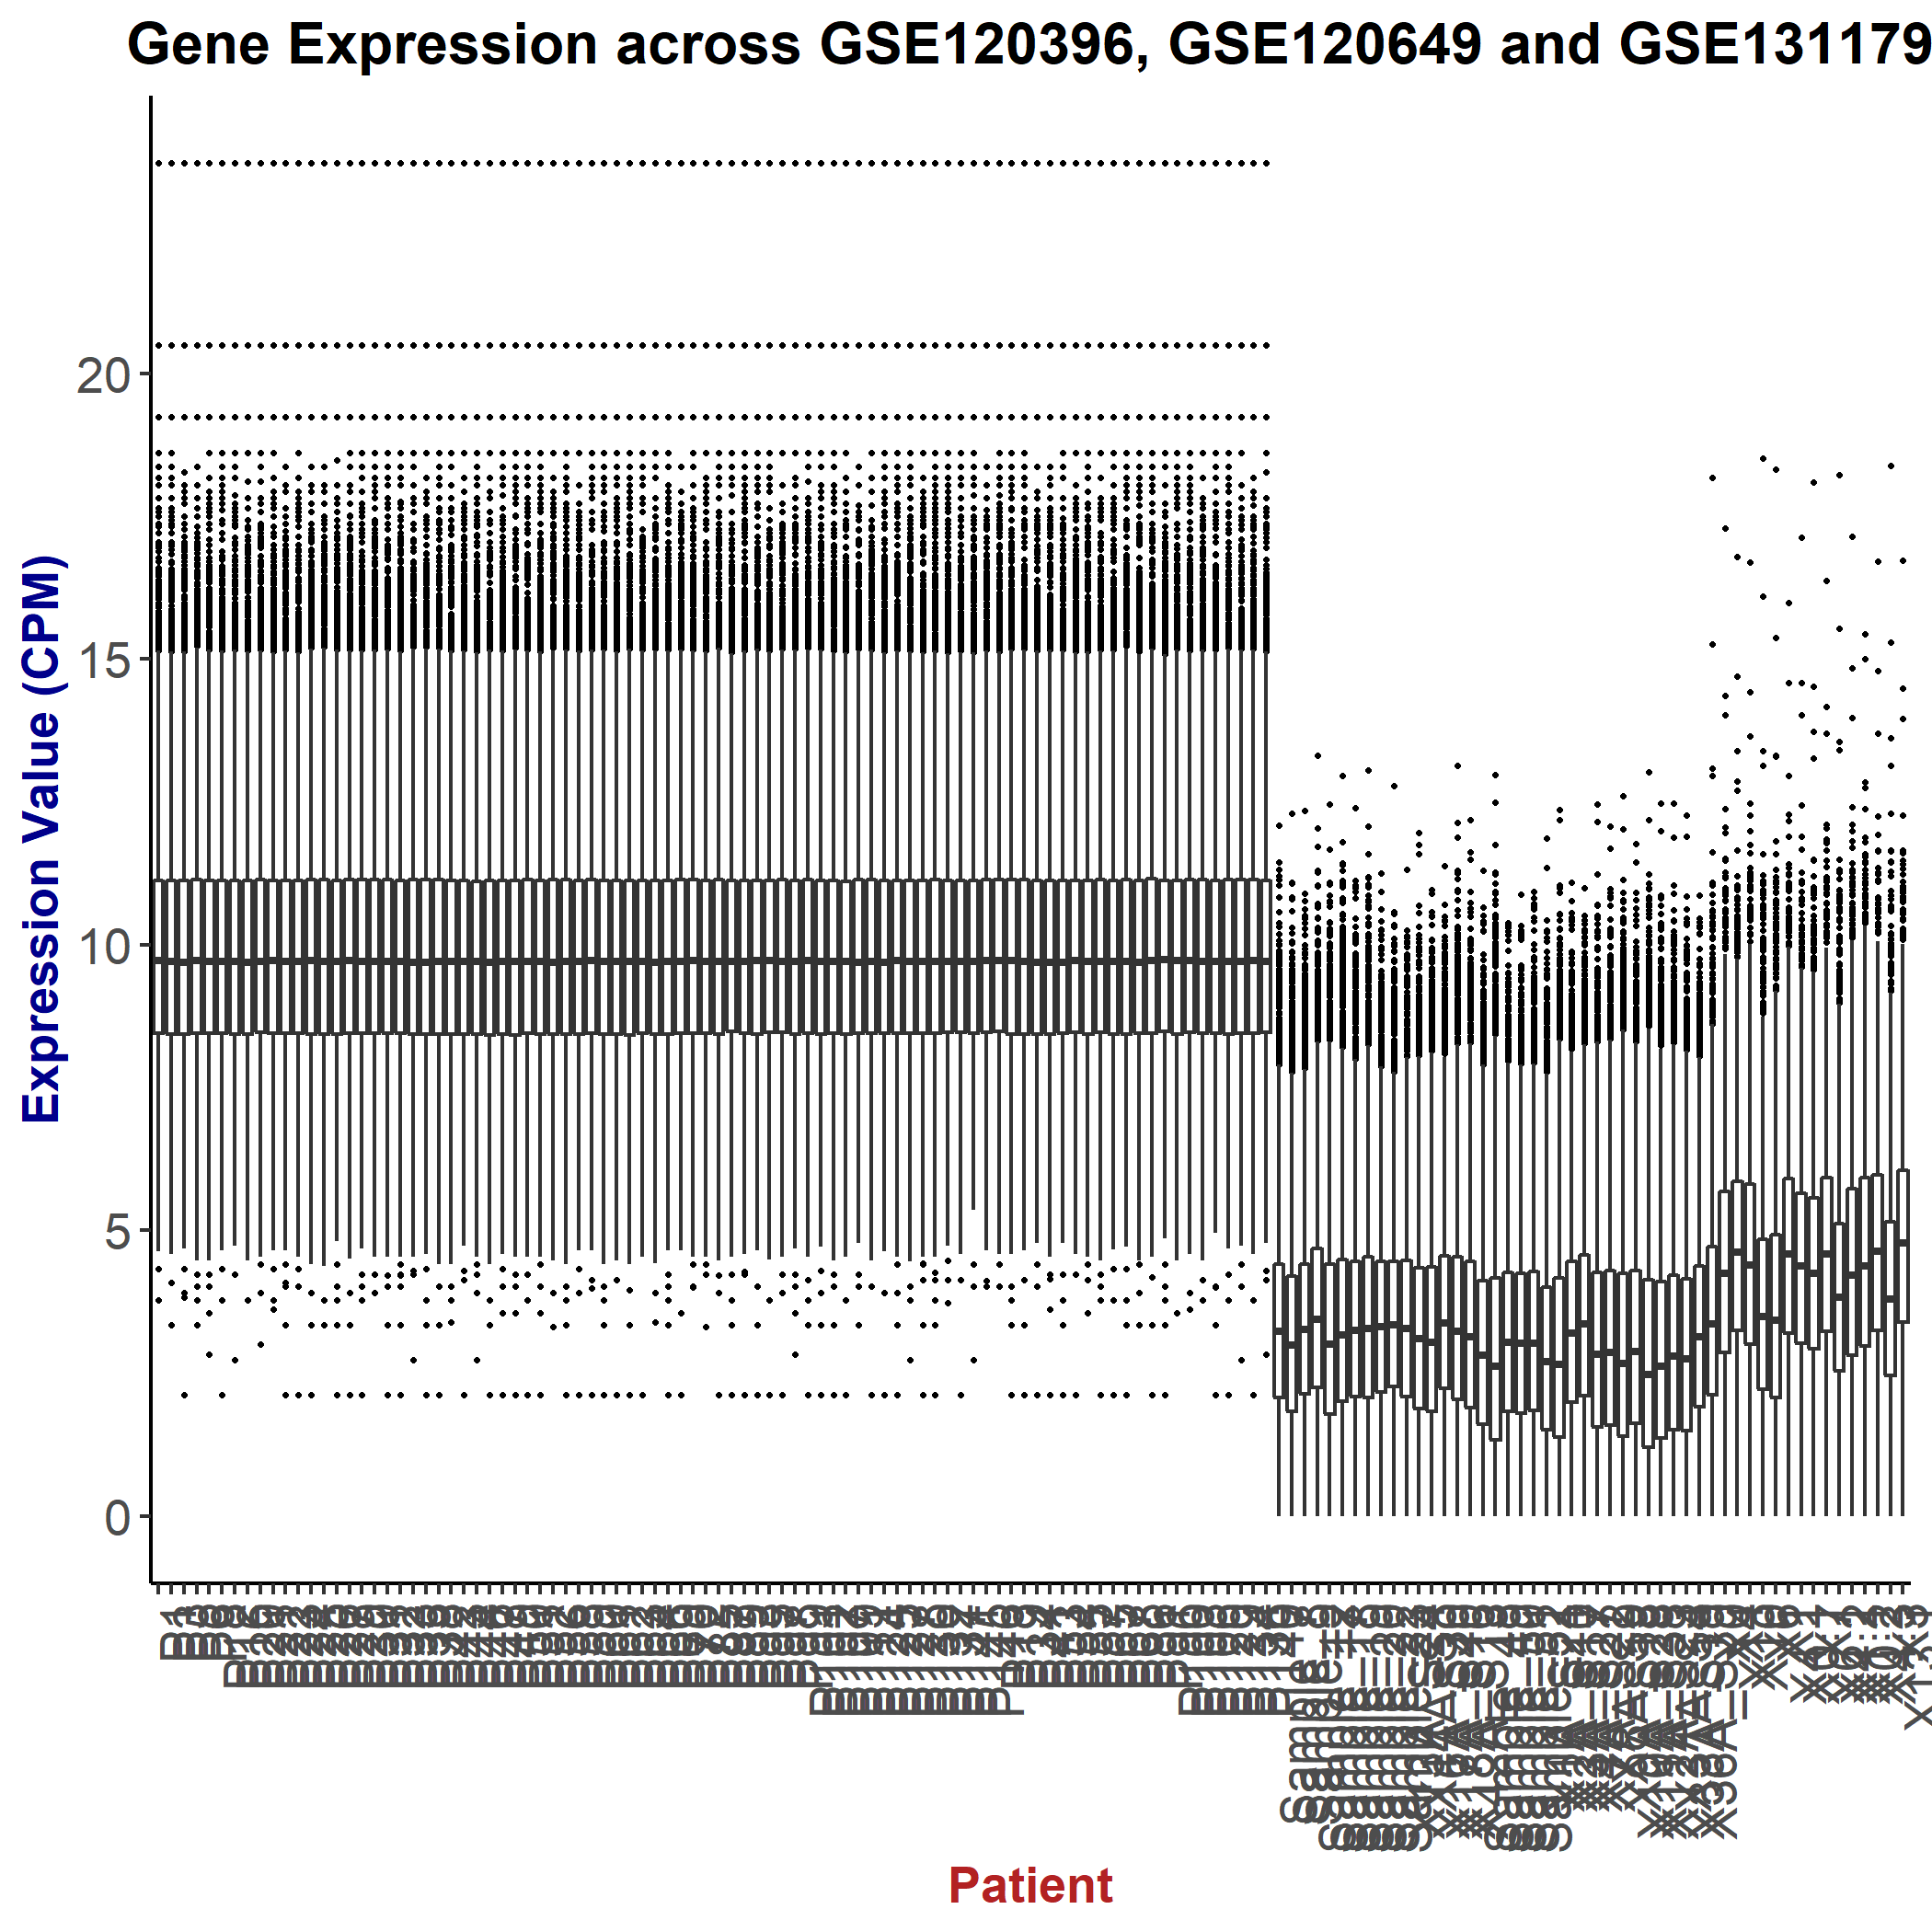
\includegraphics[width=200px]{images/part1merged} \end{center}

It can be demonstrated from the boxplots above that GSE120649 and
GSE131179 had a lower expression level than GSE120396. A possible method
to account for this is to perform quantile normalisation on the merged
data.

Quantile normalization is one of the most widely adopted pre-processing
methods for analysing RNA-Seq data - it reduces batch effect and
technological noise by scaling the variables to have values between 0
and 1, ensuring that the distribution of gene expressions from each
dataset are the same. This potentially allows for more robust
predictions that can be generalised to different sequencing platforms
(Qiu et al., 2013).

\begin{center}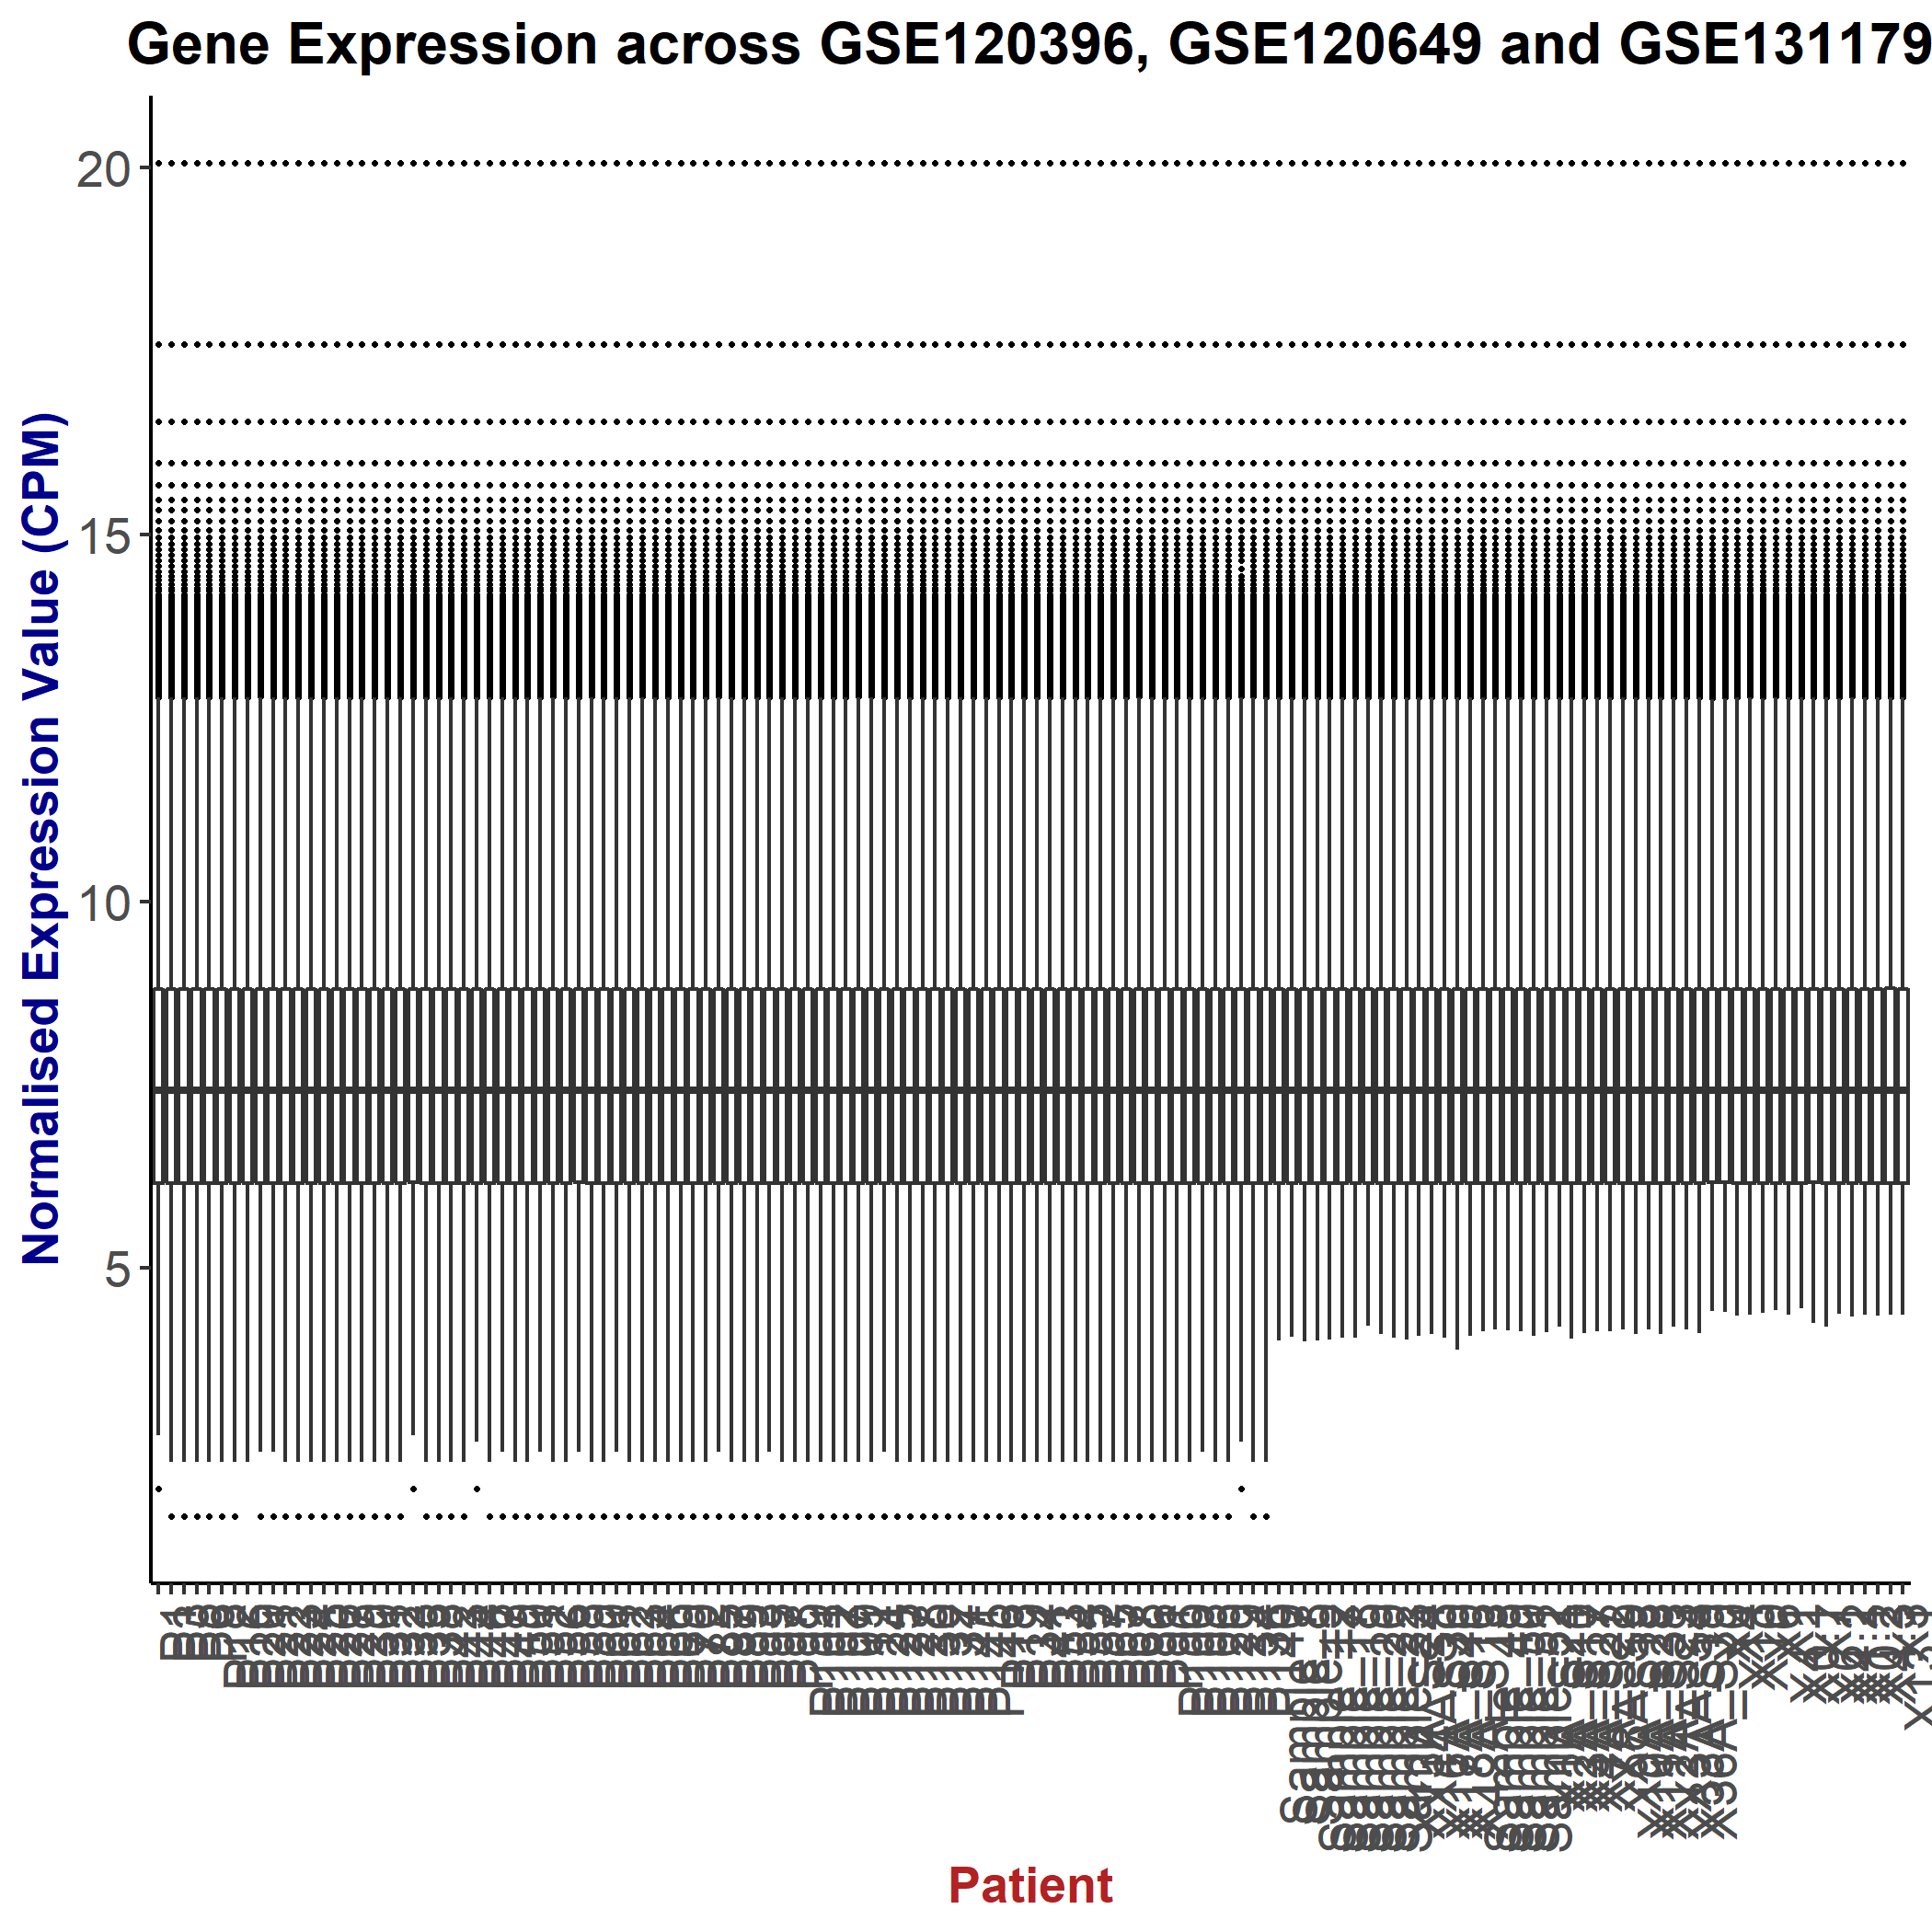
\includegraphics[width=200px]{images/part1merged_norm} \end{center}

As seen above from the boxplot above, performing quantile normalisation
had a substantial effect on gene expression distribution - the data from
all three merged studies appear normalised with similar medians around
10.

\hypertarget{part-2.-estimating-time-to-de-novo-dsa-presence}{%
\subsubsection{\texorpdfstring{Part 2. Estimating Time to \emph{de novo}
DSA
Presence}{Part 2. Estimating Time to de novo DSA Presence}}\label{part-2.-estimating-time-to-de-novo-dsa-presence}}

The eplet mismatch dataset was provided by Dr.~Germaine Wong from the
University of Sydney. Based on previous research studies conducted, it
was found that there was no significant correlation between BMI category
and graft survival (Papalia et al., 2010). Thus, we focused only on
using age and gender as phenotypic information when stratifying the
data.

Each transplant recipient from the dataset was categorised into a
certain age group (i.e. `25-35','36-45', and `46-55'), and whether they
had less-than or greater-than-or-equal-to 30 Class II eplet mismatches
(30 was approximately the median number of Class II eplet mismatches).

\begin{Shaded}
\begin{Highlighting}[]
\NormalTok{survdt_m <-}\StringTok{ }\NormalTok{survdt_m }\OperatorTok\StringTok{ }
\StringTok{    }\KeywordTok{mutate}\NormalTok{(}\DataTypeTok{agetxn =} \KeywordTok{case_when}\NormalTok{(agetxn }\OperatorTok{>=}\StringTok{ }
\StringTok{        }\DecValTok{25} \OperatorTok{&}\StringTok{ }\NormalTok{agetxn }\OperatorTok{<=}\StringTok{ }
\StringTok{        }\DecValTok{35} \OperatorTok{~}\StringTok{ "25 - 35"}\NormalTok{, }
\NormalTok{        agetxn }\OperatorTok{>=}\StringTok{ }\DecValTok{36} \OperatorTok{&}\StringTok{ }
\StringTok{            }\NormalTok{agetxn }\OperatorTok{<=}\StringTok{ }
\StringTok{                }\DecValTok{45} \OperatorTok{~}\StringTok{ }
\StringTok{            "36 - 45"}\NormalTok{, }
\NormalTok{        agetxn }\OperatorTok{>=}\StringTok{ }\DecValTok{46} \OperatorTok{&}\StringTok{ }
\StringTok{            }\NormalTok{agetxn }\OperatorTok{<=}\StringTok{ }
\StringTok{                }\DecValTok{55} \OperatorTok{~}\StringTok{ }
\StringTok{            "46 - 55"}\NormalTok{))}

\NormalTok{survdt_m <-}\StringTok{ }\NormalTok{survdt_m }\OperatorTok\StringTok{ }
\StringTok{    }\KeywordTok{mutate}\NormalTok{(}\DataTypeTok{MM =} \KeywordTok{case_when}\NormalTok{(MM }\OperatorTok{<=}\StringTok{ }
\StringTok{        }\DecValTok{30} \OperatorTok{~}\StringTok{ "<= 30 MM"}\NormalTok{, }
\NormalTok{        MM }\OperatorTok{>}\StringTok{ }\DecValTok{30} \OperatorTok{~}\StringTok{ "> 30 MM"}\NormalTok{, }
\NormalTok{        ))}
\end{Highlighting}
\end{Shaded}

From this, a Survival object was created based on these age/gender
subpopulations stratified by their number of Class II mismatches
(\textless{} 30 or \textgreater{}= 30), with the event as the presence
of DSA and the time taken for the event to occur.

\begin{Shaded}
\begin{Highlighting}[]
\CommentTok{# E.g. Selecting a}
\CommentTok{# male aged 46 - 55}
\CommentTok{# years}
\NormalTok{user_survdt =}\StringTok{ }\NormalTok{survdt_m }\OperatorTok\StringTok{ }
\StringTok{    }\NormalTok{dplyr}\OperatorTok{::}\KeywordTok{filter}\NormalTok{(Gender }\OperatorTok{==}\StringTok{ }
\StringTok{        "Male"}\NormalTok{, Age }\OperatorTok{==}\StringTok{ }
\StringTok{        "46 - 55"}\NormalTok{)}
\end{Highlighting}
\end{Shaded}

The visualisation of the survival curve for the subpopulation was
represented through a Kaplan-Meier curve.

\hypertarget{part-3.-predicting-operational-tolerance}{%
\subsubsection{Part 3. Predicting Operational
Tolerance}\label{part-3.-predicting-operational-tolerance}}

To predict operational tolerance, we collected the GSE22229 dataset
which contained raw CEL files pertaining to the gene expression for
patients that were either tolerant or not.

CEL files are created by the Affymetrix DNA microarray image analysis
software, and contain estimated probe (sequence of DNA base pairs)
intensity values extracted from Affymetrix Genechips. Each probe was
mapped to a specific gene symbol using the GPL570 Chip Description File
(CDF).

Since the data is in the newer Affymetrix Arrays format (Gene ST
arrays), we utilised the \texttt{oligo} library to read a list of CEL
files. This list was then converted from an AffyBatch object into an
ExpressionSet (i.e.~gene expression) using the \texttt{rma} function
from the \texttt{pd.mogene.2.0.st} library. The \texttt{rma} function,
short for \emph{Robust Multichip Average}, also simultaneously
log\textasciitilde{}2 transforms and normalises the gene expressions.

\begin{Shaded}
\begin{Highlighting}[]
\KeywordTok{setwd}\NormalTok{(}\StringTok{"data/GSE22229_RAW/"}\NormalTok{)}
\NormalTok{celFiles <-}\StringTok{ }\KeywordTok{list.celfiles}\NormalTok{()}
\NormalTok{affyRaw <-}\StringTok{ }\KeywordTok{read.celfiles}\NormalTok{(celFiles)}
\NormalTok{eset <-}\StringTok{ }\KeywordTok{rma}\NormalTok{(affyRaw)}

\KeywordTok{setwd}\NormalTok{(}\StringTok{"../../"}\NormalTok{)}
\KeywordTok{write.exprs}\NormalTok{(eset, }\DataTypeTok{file =} \StringTok{"tolerance.txt"}\NormalTok{)}
\NormalTok{my_frame <-}\StringTok{ }\KeywordTok{data.frame}\NormalTok{(}\KeywordTok{exprs}\NormalTok{(eset))}
\KeywordTok{write.table}\NormalTok{(my_frame, }
    \DataTypeTok{file =} \StringTok{"tolerance.txt"}\NormalTok{, }
    \DataTypeTok{sep =} \StringTok{"}\CharTok{\textbackslash{}t}\StringTok{"}\NormalTok{)}
\end{Highlighting}
\end{Shaded}

After converting our ExpressionSet object into a dataframe, we then
investigated the gene expression distribution amongst patients using a
boxplot to ensure that the data has been normalised and can be used for
further processing.

\begin{center}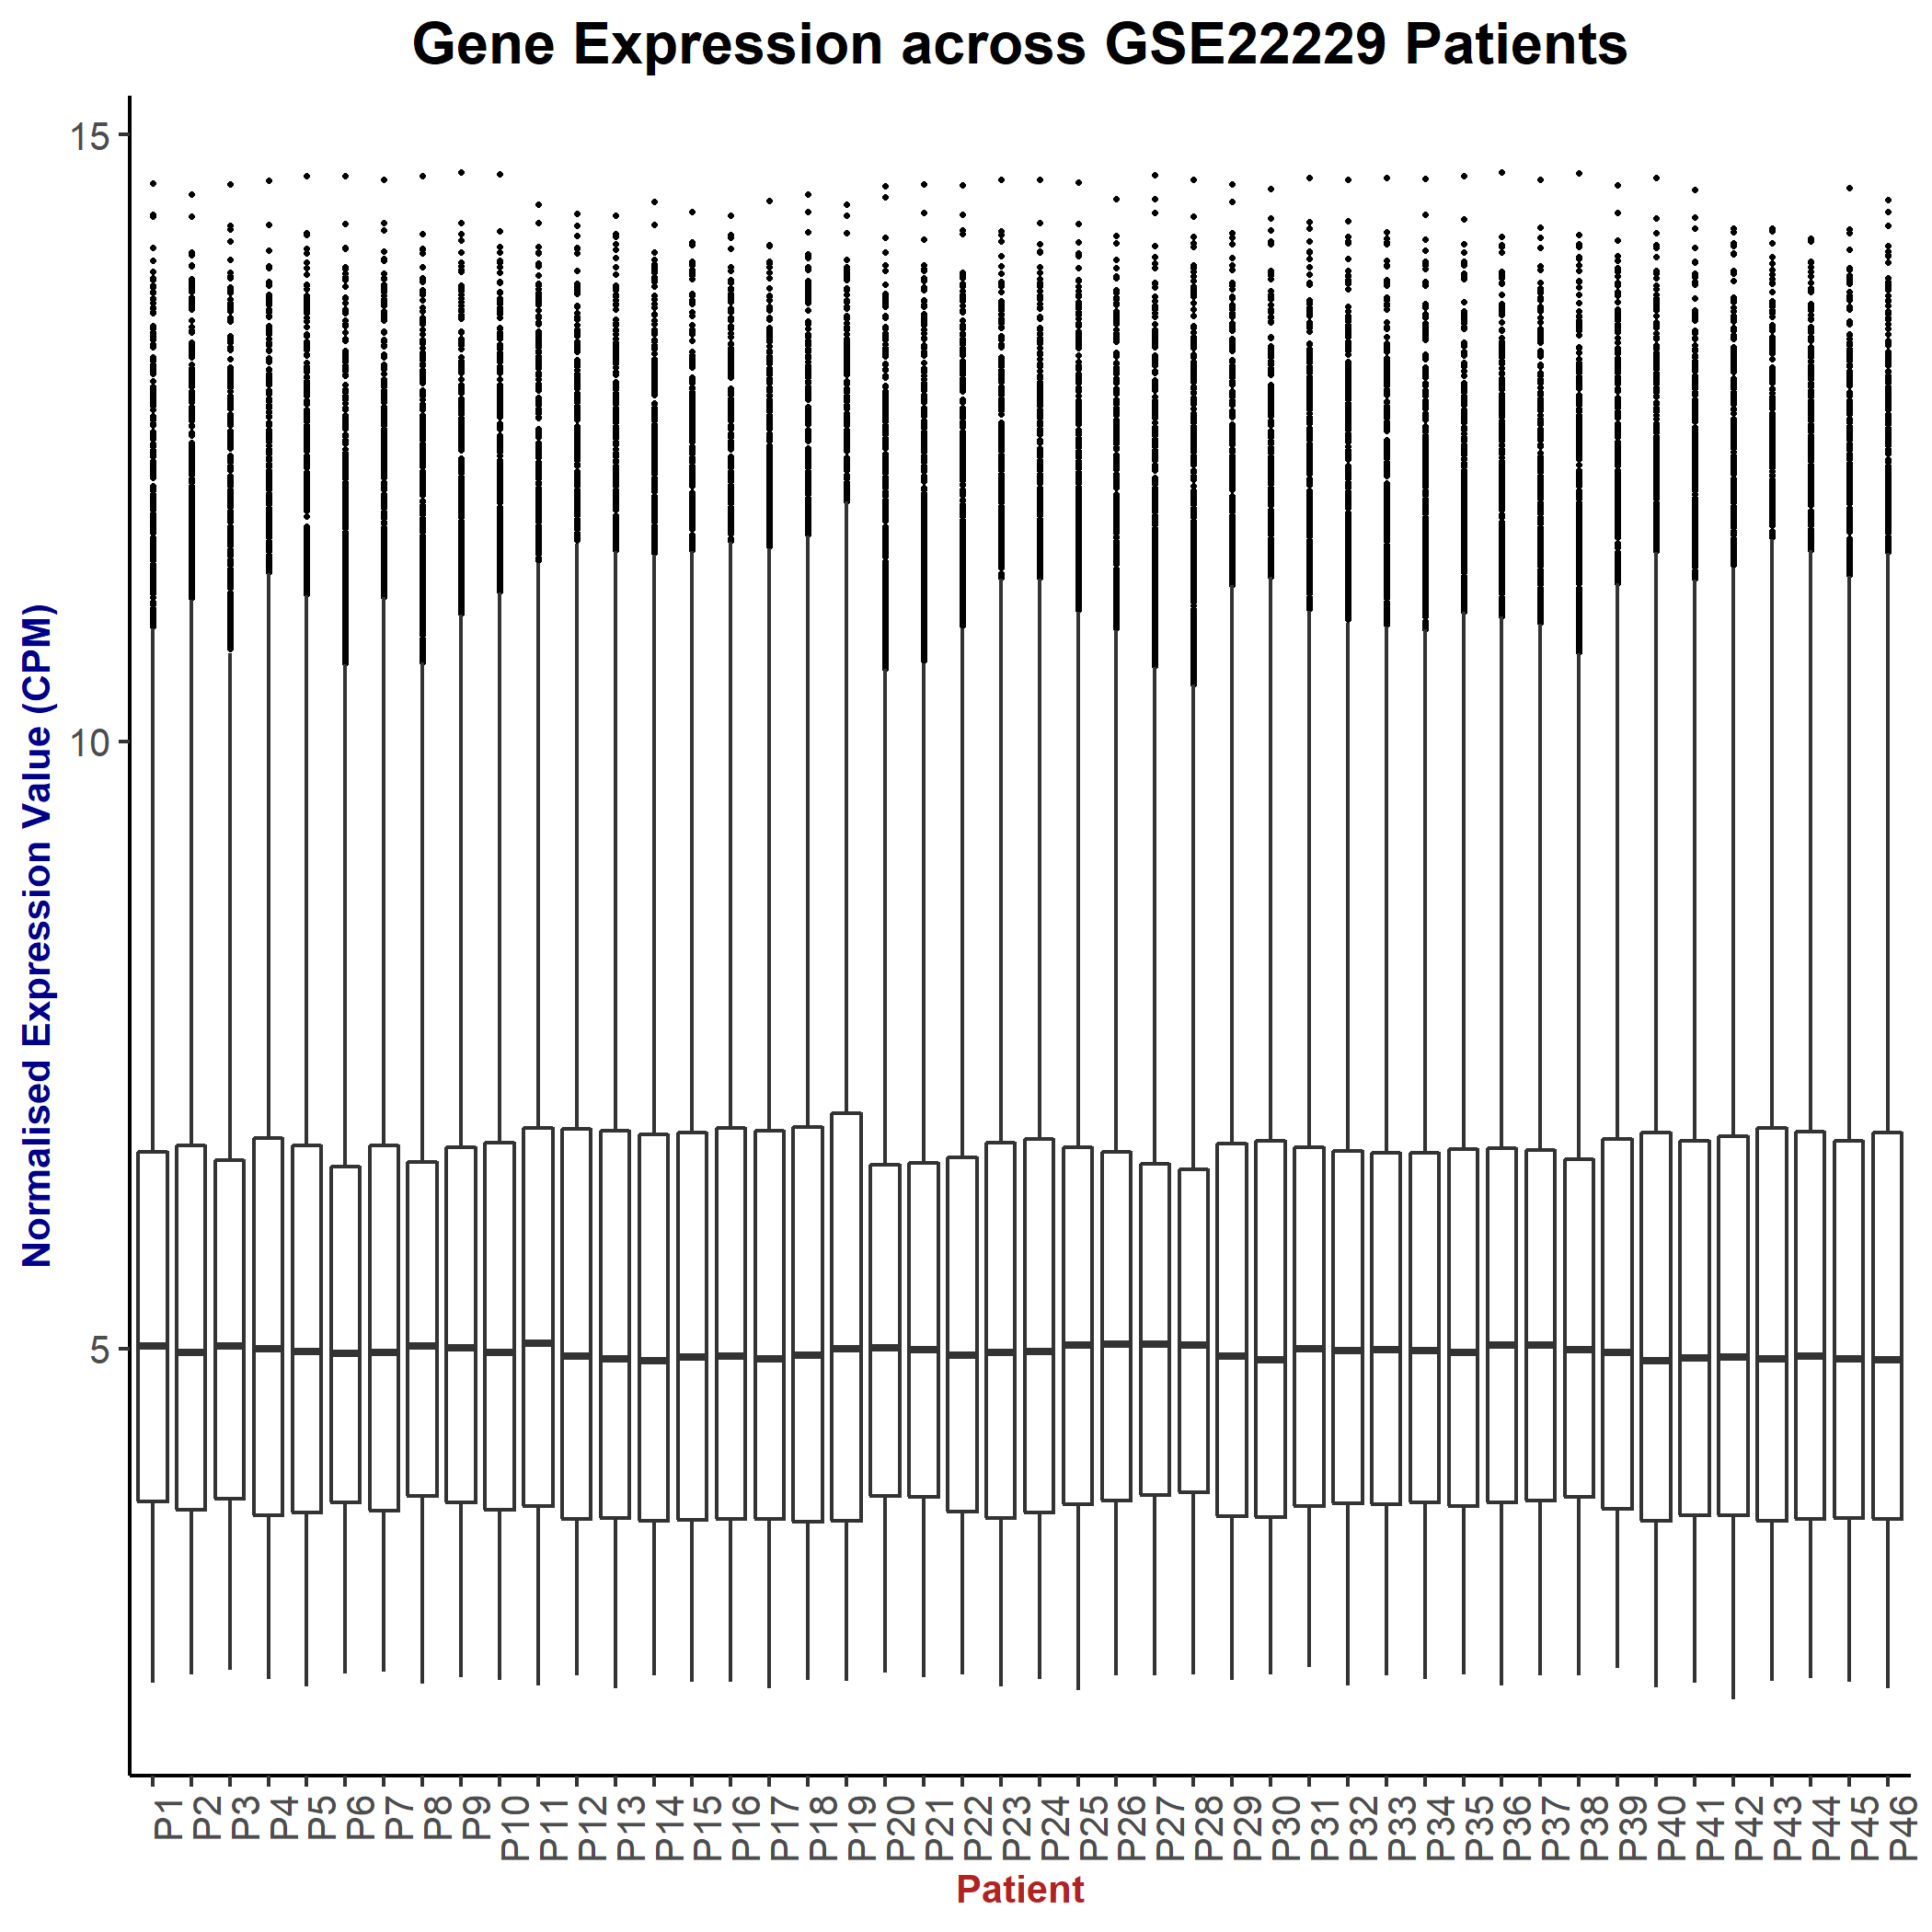
\includegraphics[width=200px]{images/part3boxplot} \end{center}

The boxplot above demonstrates strong similarity in gene expression
between patients and so our dataframe can be further analysed without
concern of batch effects between sample measurements.

After quantile normalization and batch effect removal, we performed
feature selection. Firstly, genes that were lowly expressed in both
groups were removed by using the \texttt{filterByExpr()} function from
the \texttt{edgeR} package; these genes do not provide much biological
meaning and removing them allows for less statistical tests to be
performed, as well as allowing greater reliability in observing the
variance between different groups (Law et al., 2018)

We then selected the most differentially expressed genes between the two
groups using multiple \emph{t}-tests from the \texttt{limma} package.
Finally, a review by Massart et al. (2017) suggested a collection of
genes that were highly differential between tolerant and normal
patients, and so these were also added to our final training dataset (if
they weren't already filtered for previously).

\hypertarget{evaluation-strategies}{%
\subsection{Evaluation Strategies}\label{evaluation-strategies}}

We decided to implement penalised logistic regression methods when
creating separate predictive models for Part 1 and Part 3 of our risk
calculator. Logistic regression was utilised as it provides a
probabilistic output for a specific risk, which may be more informative
than a binary outcome. Furthermore, the penalised nature of some methods
(e.g.~Ridge, LASSO, Elastic Net) can address the overfitting or
multicollinearity issue prevalent in large \emph{p}, small \emph{n}
situations in gene expression data.

The models for Part 1 and Part 3 were trained using their respective
pre-processed data onto a 50-repeated 5-fold cross validation (CV)
procedure. The performance of our models in predicting the CV test-set
under Ridge, LASSO and Elastic Net methods were evaluated using three
primary metrics: accuracy, AUC and the Brier Score.

In the case of class imbalance within the training dataset, the accuracy
metric may suggest an inflated performance. As such, the AUC and Brier
Score were also calculated.

• The AUC is a more robust metric with less bias to class size. Briefly,
it can be thought of as the probability that a true-positive sample
(e.g.~AR patient) has a greater predicted risk than a true-negative
sample (e.g.~normal patient).

• The Brier Score meanwhile complements the AUC by checking that the
predicted risk of a sample is actually similar to the true value. For
example, in a true-positive case (i.e.~label = 1) with a predicted risk
of 0.8, the Brier Score quantitatively measure how close the 0.8 value
is to 1. Better predictions are reflected as a lower Brier Score.

To select our final models for Part 1 and Part 3 respectively, we
evaluated the accuracy, AUC, and Brier Score from different penalised
models (Ridge, LASSO, and Elastic Net) using boxplot visualisations.

For Part 2, since we are not predicting the probability of graft failure
over time, there was no need to build and train a model.

\hypertarget{model-selection}{%
\subsection{Model Selection}\label{model-selection}}

To select the optimal number of features (i.e.~genes) for our model, the
CV accuracy using the top 5 up to the top 120 most significant genes
were calculated respectively.

For Part 1, high LASSO accuracy was seen around \emph{n} = 12 with 79\%.
However, this may not be robust when applied to real world data. In
particular, it is unlikely that AR is caused only by the 12 genes, and
it is also unlikely that incoming patient data will have these 12
significant genes.

\begin{center}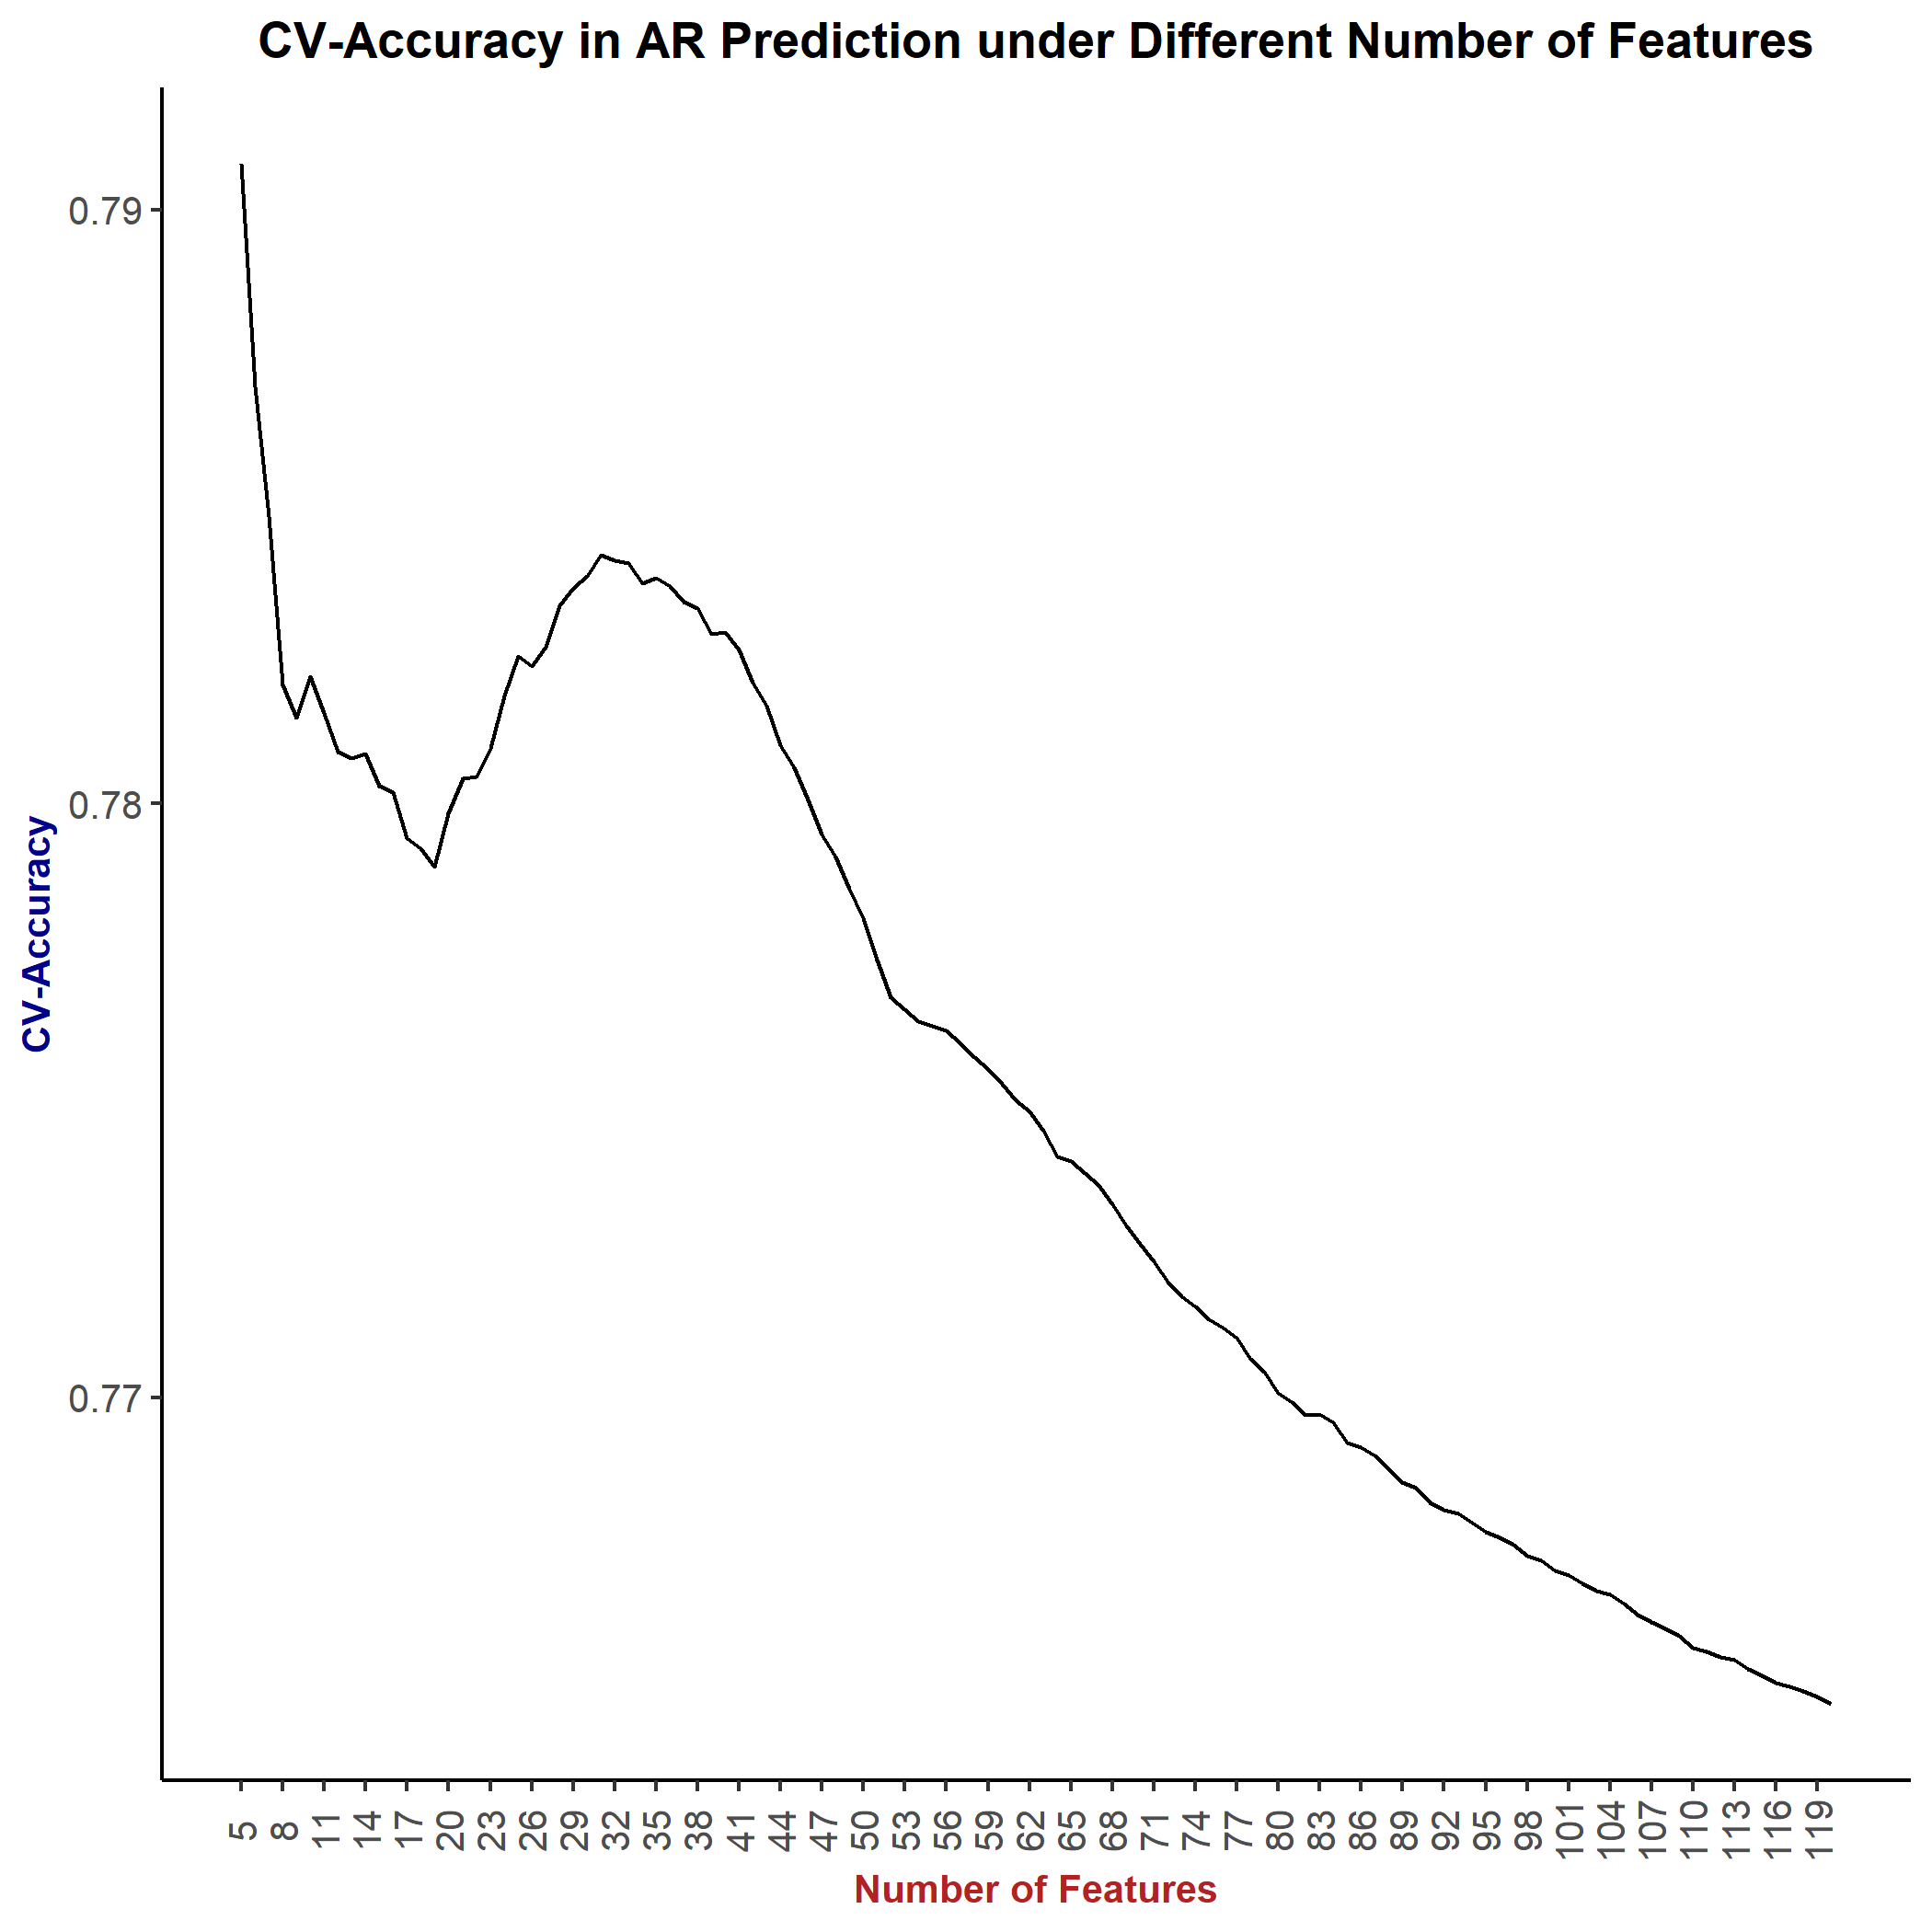
\includegraphics[width=250px]{images/part1features} \end{center}

Combined with the fact that penalised regression models can elicit
further variable reduction, the choice of using 12 genes as predictors
in our model may not be statistically wise. Hence, we decided to instead
incorporate the top 100 most significant genes into our model for Part
1, which had a CV accuracy of 77\%. Indeed, while this is marginally
smaller than the CV accuracy for the top 12 genes, the use of top 100
genes may be more robust to independent data. As such, we also selected
the top 100 most differentially expressed genes between OT and non-OT
patients as our features for the Part 3 model.

When evaluating the CV accuracy, AUC, and Brier Score of Ridge, LASSO,
and Elastic net, it was found that for both Part 1 and Part 3 data,
Elastic Net mostly produced the best performance based on the three
metrics. Below are the CV results from Elastic Net for both Part 1 and
Part 3 (see Appendix for Ridge and LASSO results).

\begin{center}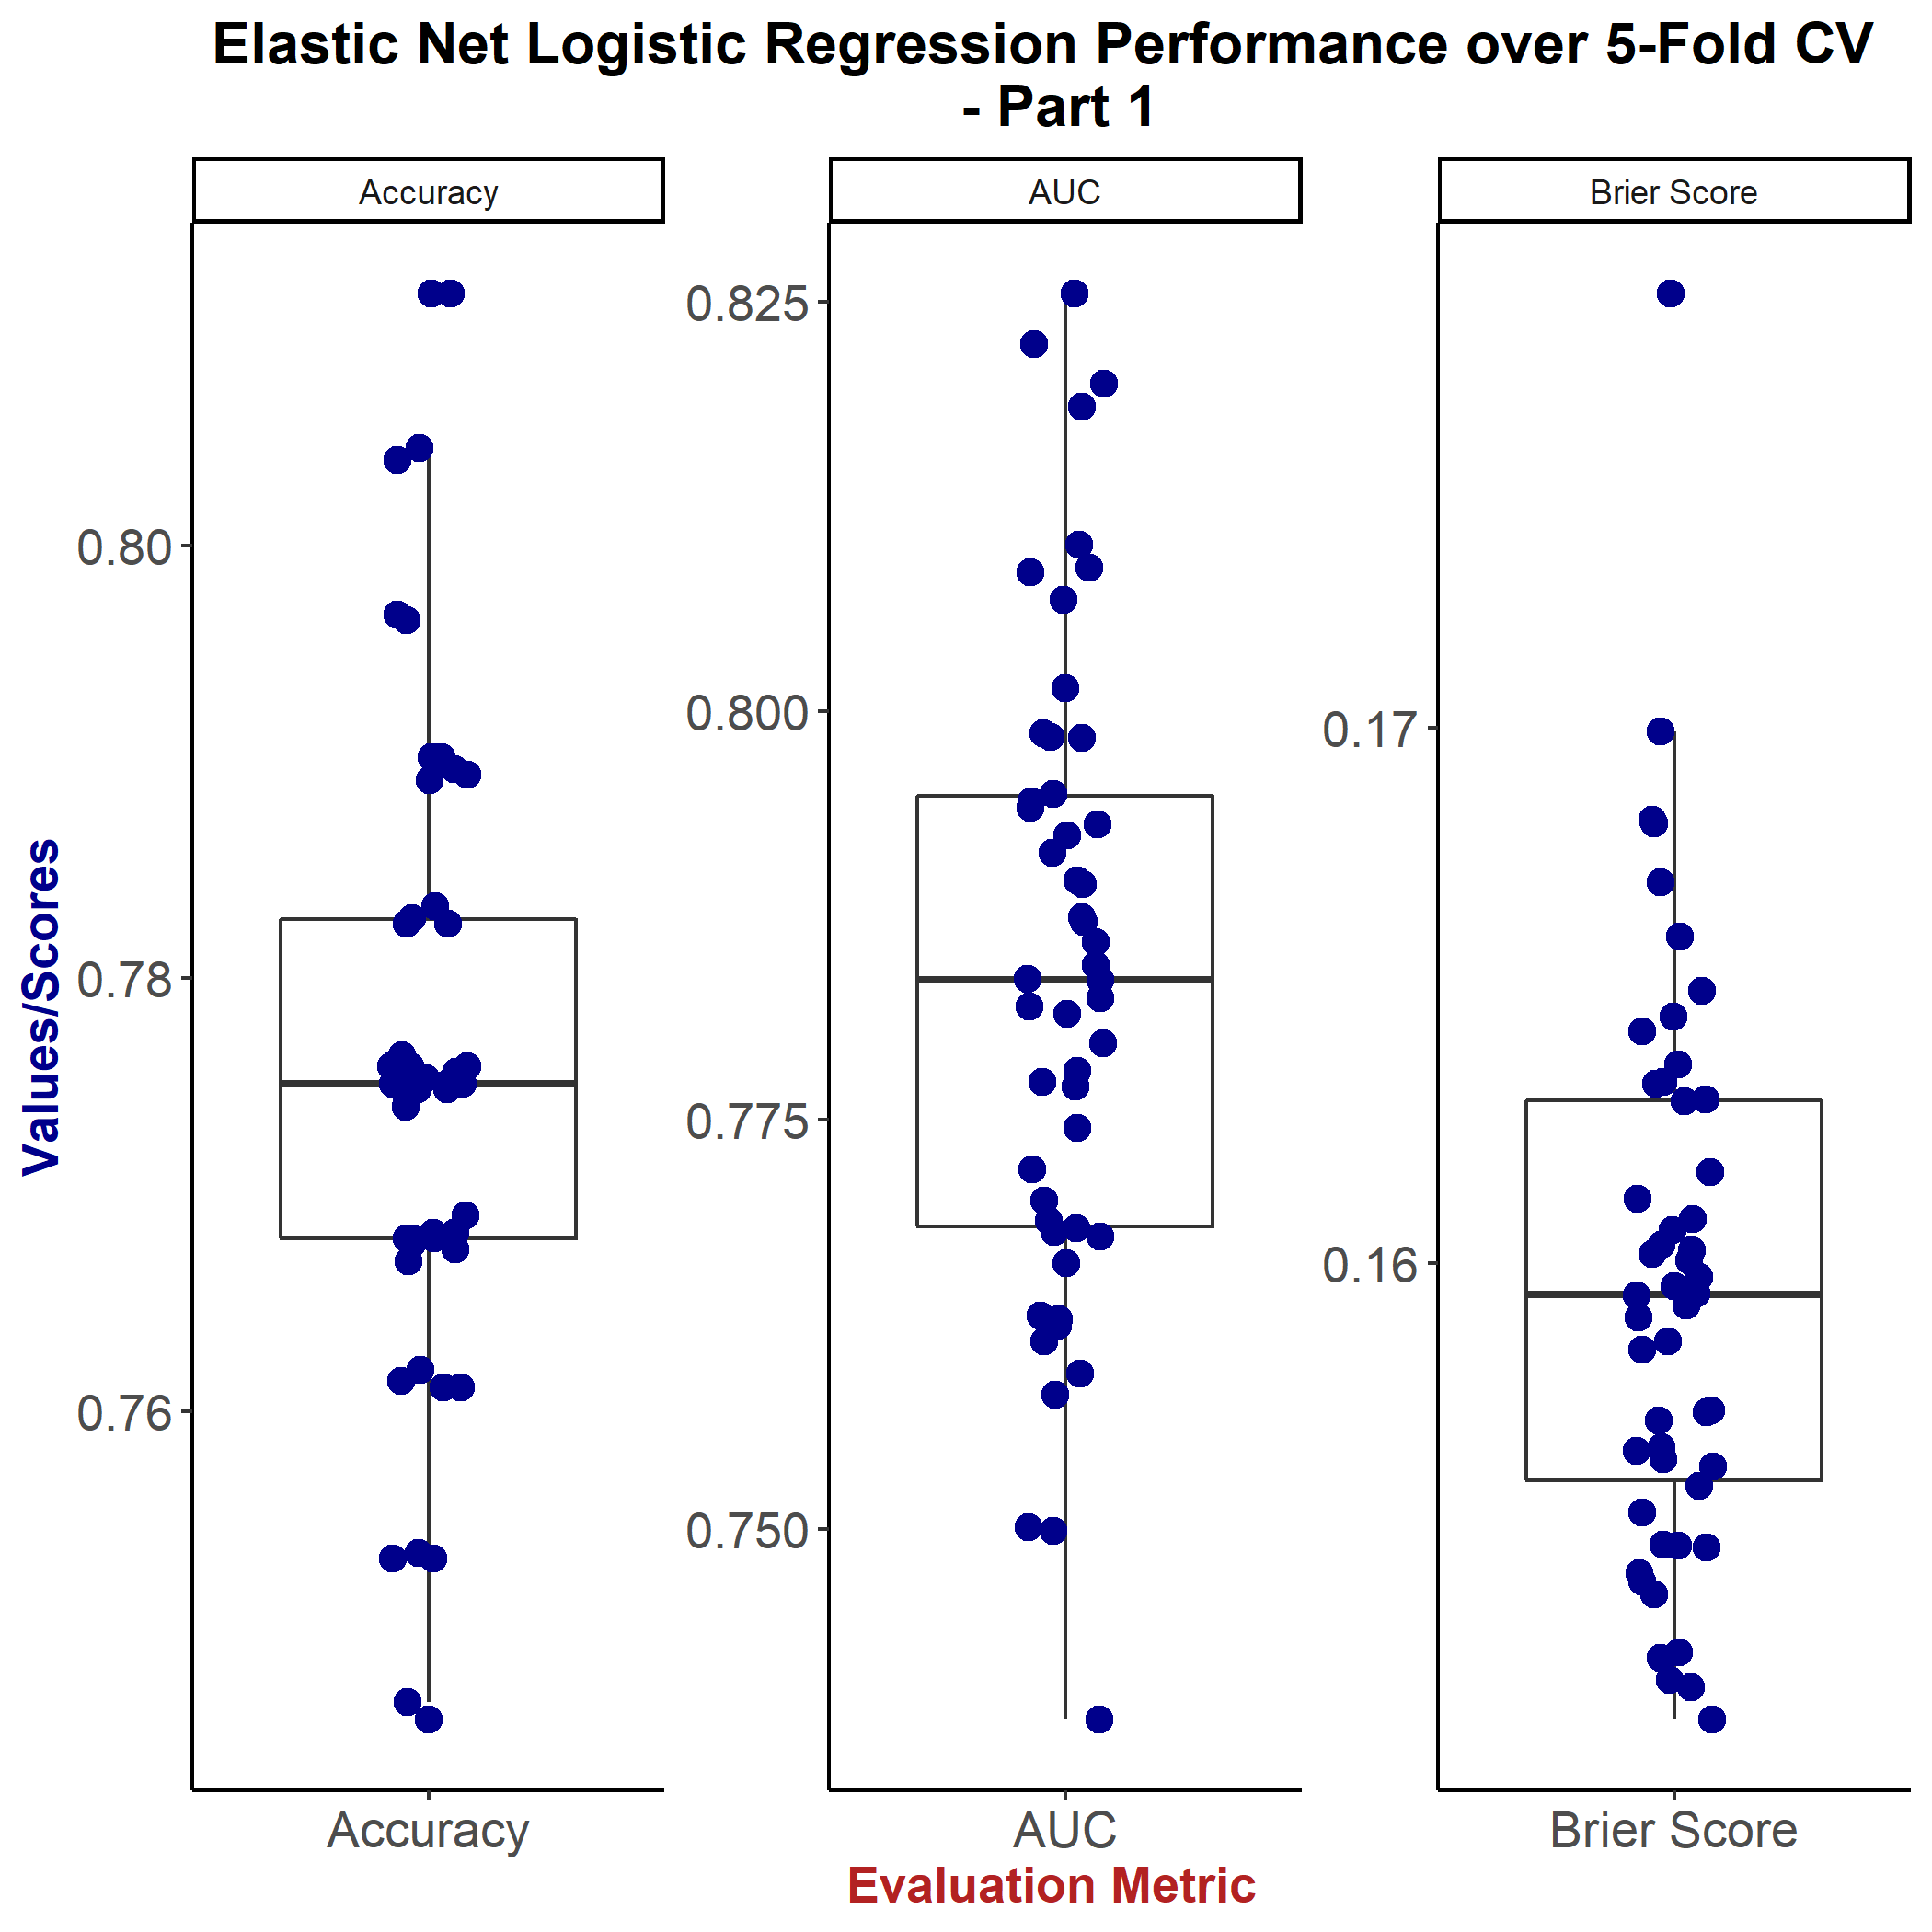
\includegraphics[width=200px]{images/part1elastic} \end{center}

\begin{center}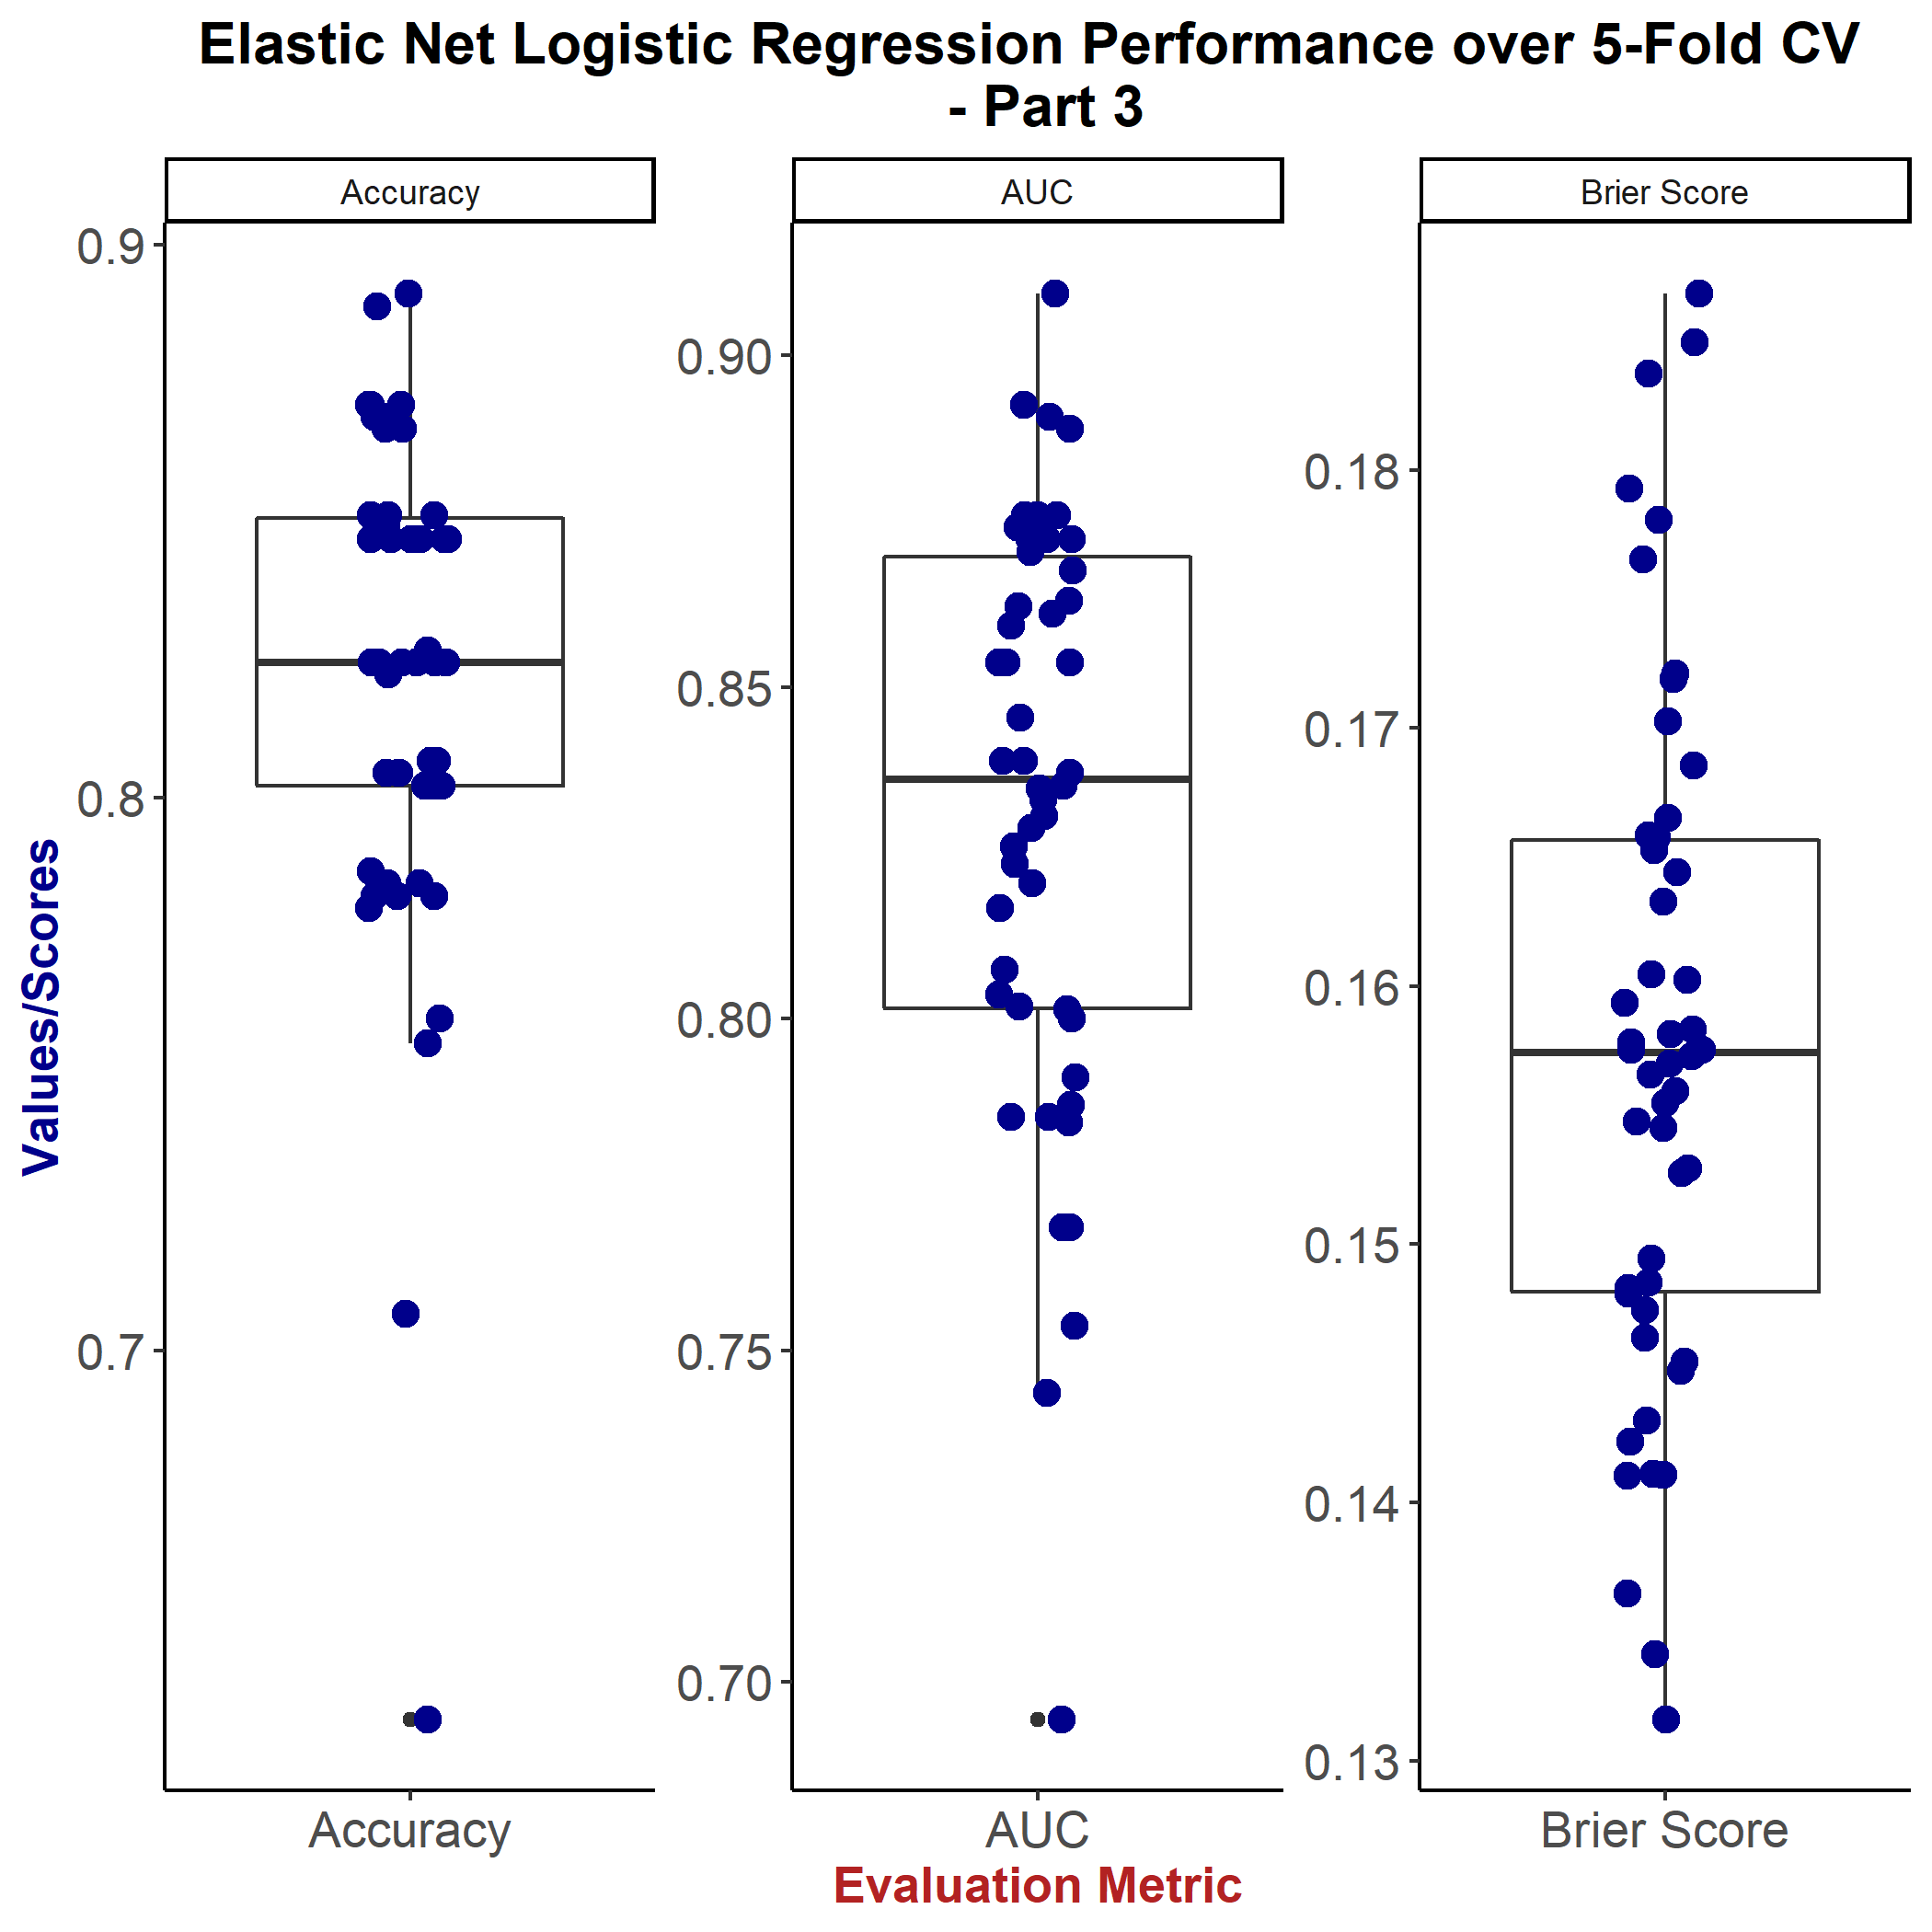
\includegraphics[width=200px]{images/part3elastic} \end{center}

Therefore, our final model for Part 1 and Part 3 separately is an
Elastic Net logistic regression model with 100 features that can address
both internal and external validity.

\hypertarget{deployment-process}{%
\subsubsection{Deployment Process}\label{deployment-process}}

Our risk calculator was deployed as an interactive Shiny application
with a simple UI for patient input. An `Information' tab (Appendix) was
also present that explains our mission, as well as providing theoretical
information about AR and OT such that patients may be more medically
informed and possibly be encouraged to demonstrate adherence and
understanding to prescriptions.

To predict the risk of acute rejection and the likelihood of the patient
relying on immunosuppression, the two trained Elastic Net models from
Part 1 and Part 3 respectively will be applied to incoming gene
expression data from the patient. Our Shiny application allows the user
to input a \emph{.csv} or \emph{.txt} file containing raw gene counts
(Appendix), which will be transformed with CPM and log\textasciitilde{}2
functions. If the input file contains Ensembl ID, our application will
automatically convert it to official gene symbols.

The inbuilt pre-processing function ensures that the app is efficient
and easy to use for practitioners, who may not be confident to transform
and process gene expression data. If all 100 genes used for the model
are present in the input data, the trained model will be used.

However, if the input data only includes a portion of the 100 filtered
genes, an alternative Elastic Net model will be trained on the spot as
mentioned in our \emph{Evaluation Strategies} section, but only on these
portions of genes as the features in the original dataset. As the
prediction from the alternative model can be different depending on the
training-test split, we use the mean of 30 repeats to increase
reliability.

The output of the risk calculator includes two colour-coded gauge plots,
showing the predicted risk for the individual, and the population risk.
This ensures that the information is easy to understand and can be
easily understood by the patient to promote shared decision making.
Below is an example output for AR prediction after patient data has been
supplied. For results in predicting immunosuppression reliance, please
see the Appendix.

\begin{center}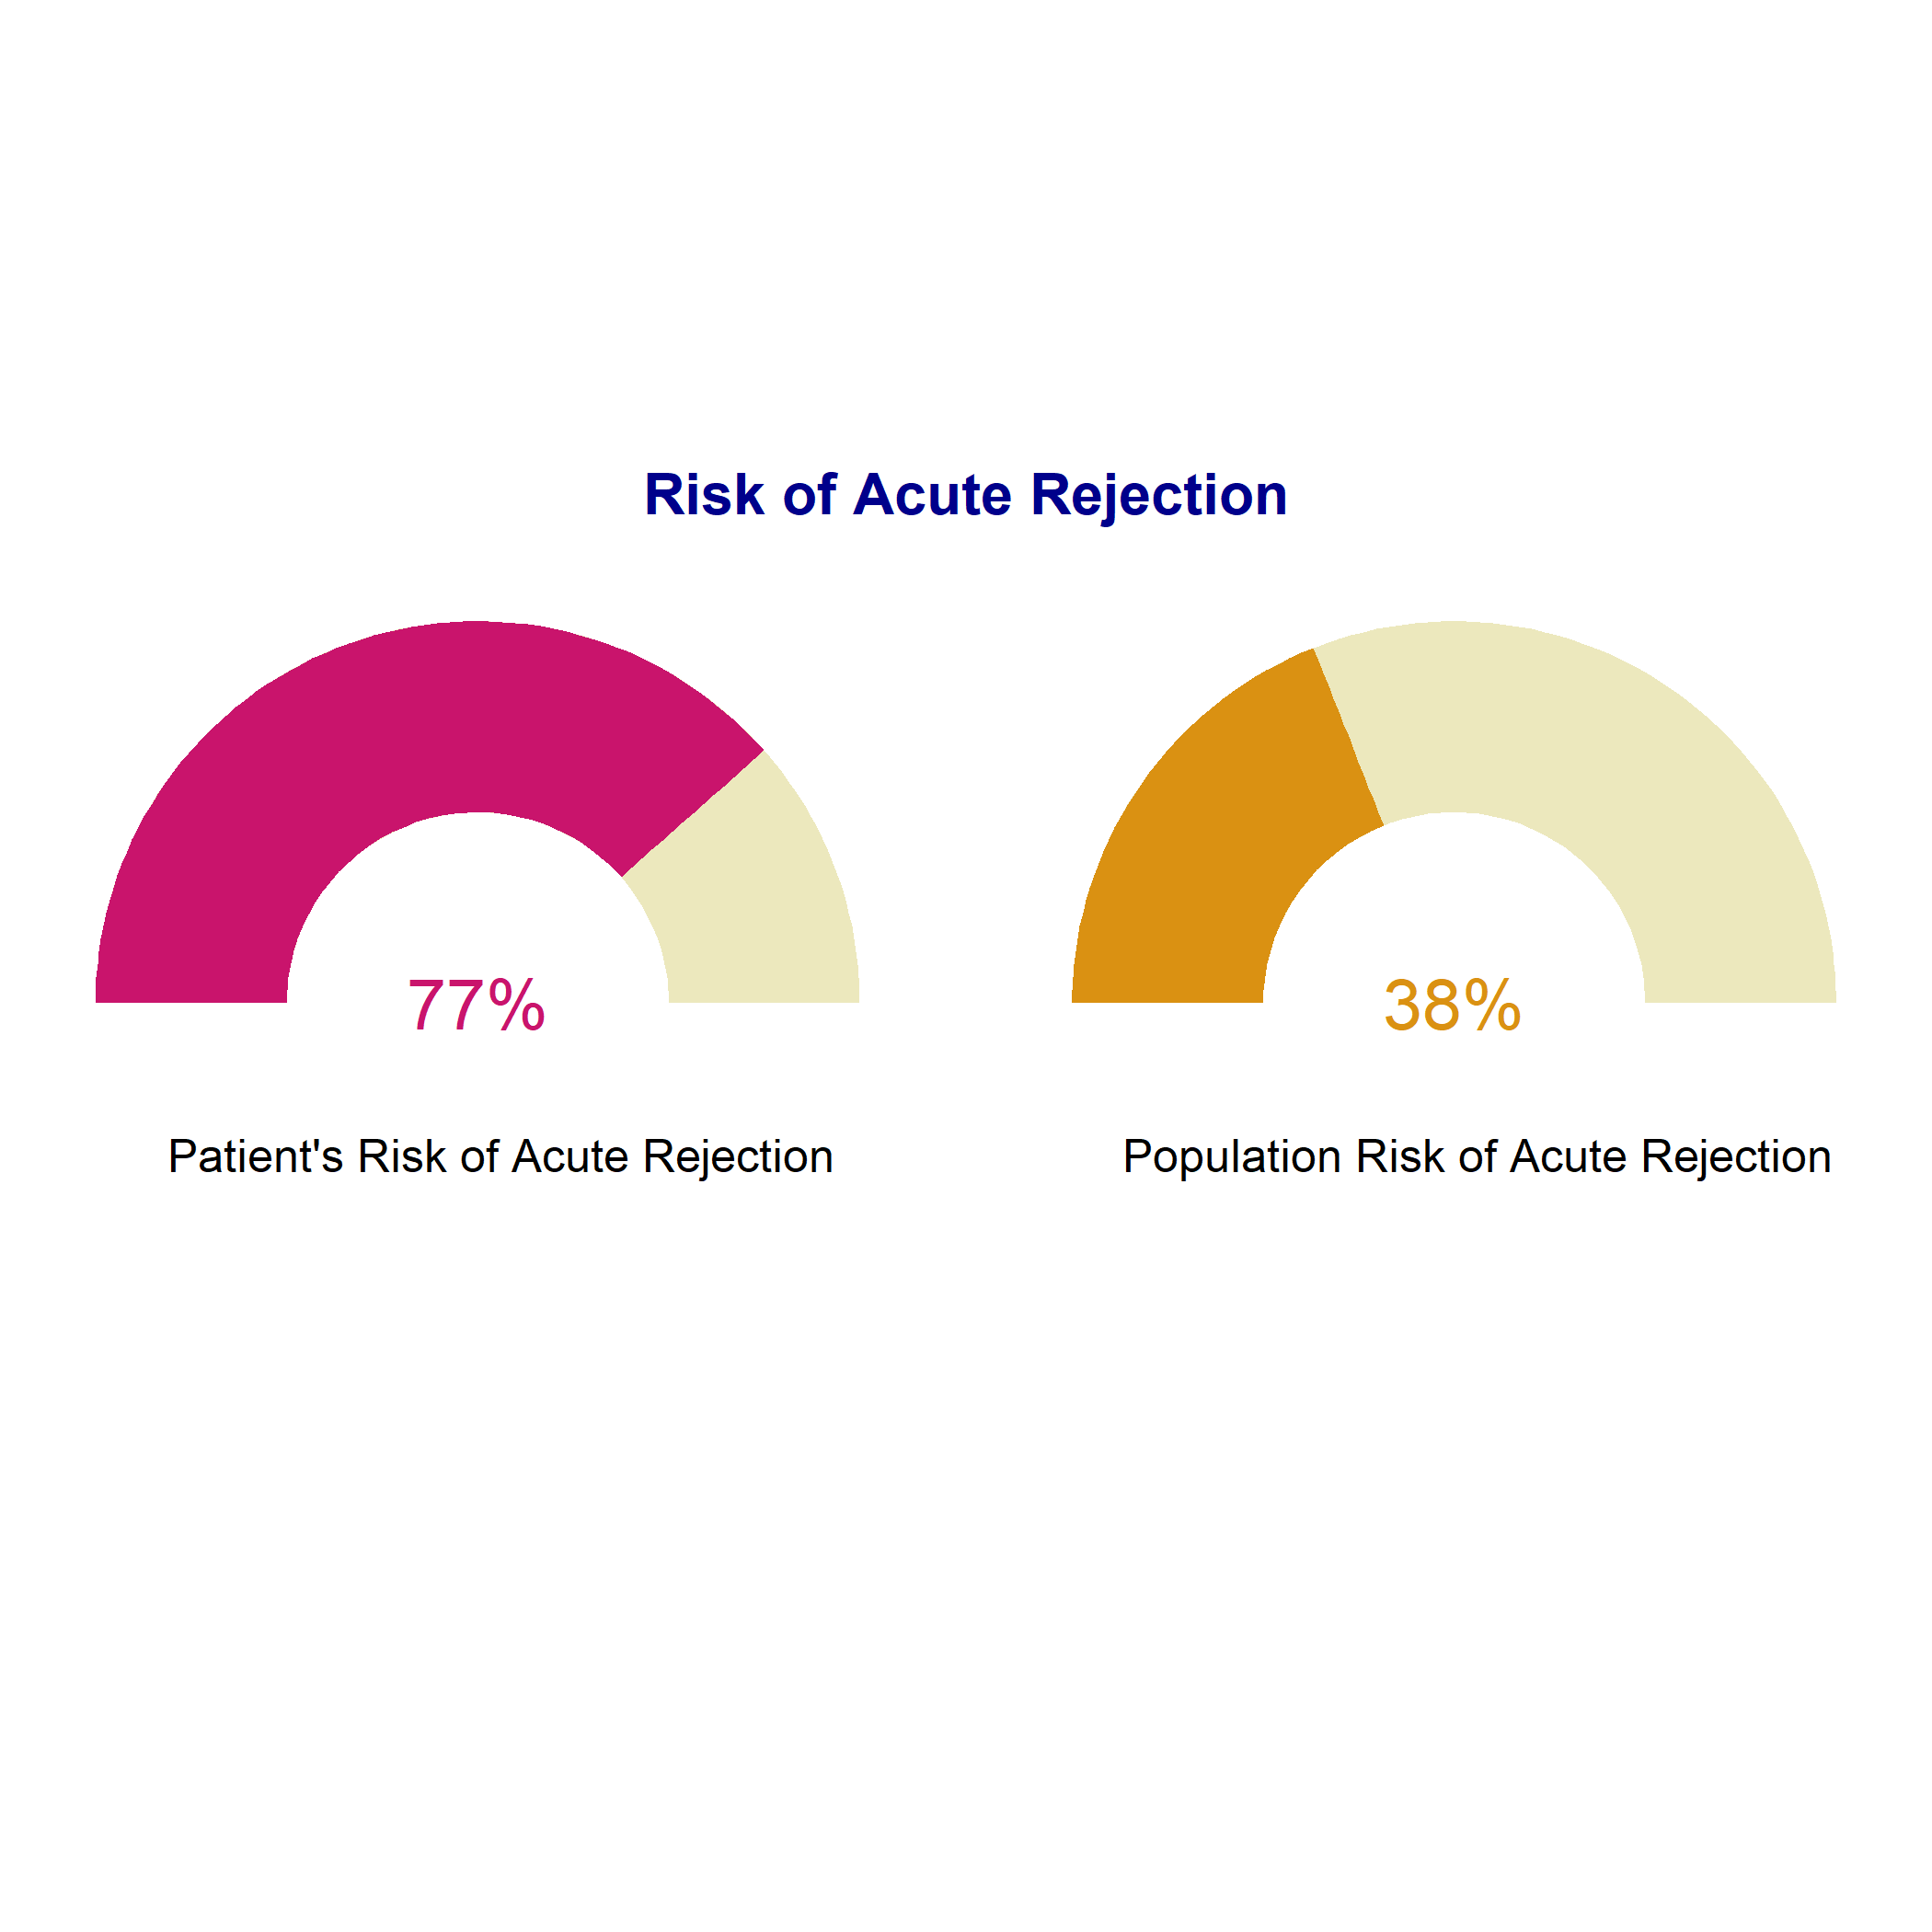
\includegraphics[width=200px]{images/part1_gauge} \end{center}

The population risk for AR were based on the findings by Menon et al.
(2017), and the percentage of the population not having OT (and thus
requiring sustained immunosuppression) were based on the review by
Newell et al. (2018)

For Part 2, a Kaplan-Meier curve was used to visualize the predictive
outcome (time to DSA presence) for a subset of a population, which in
our case was based on age and sex stratified by the potential number of
eplet mismatches the recipient may have with the donor.

\begin{center}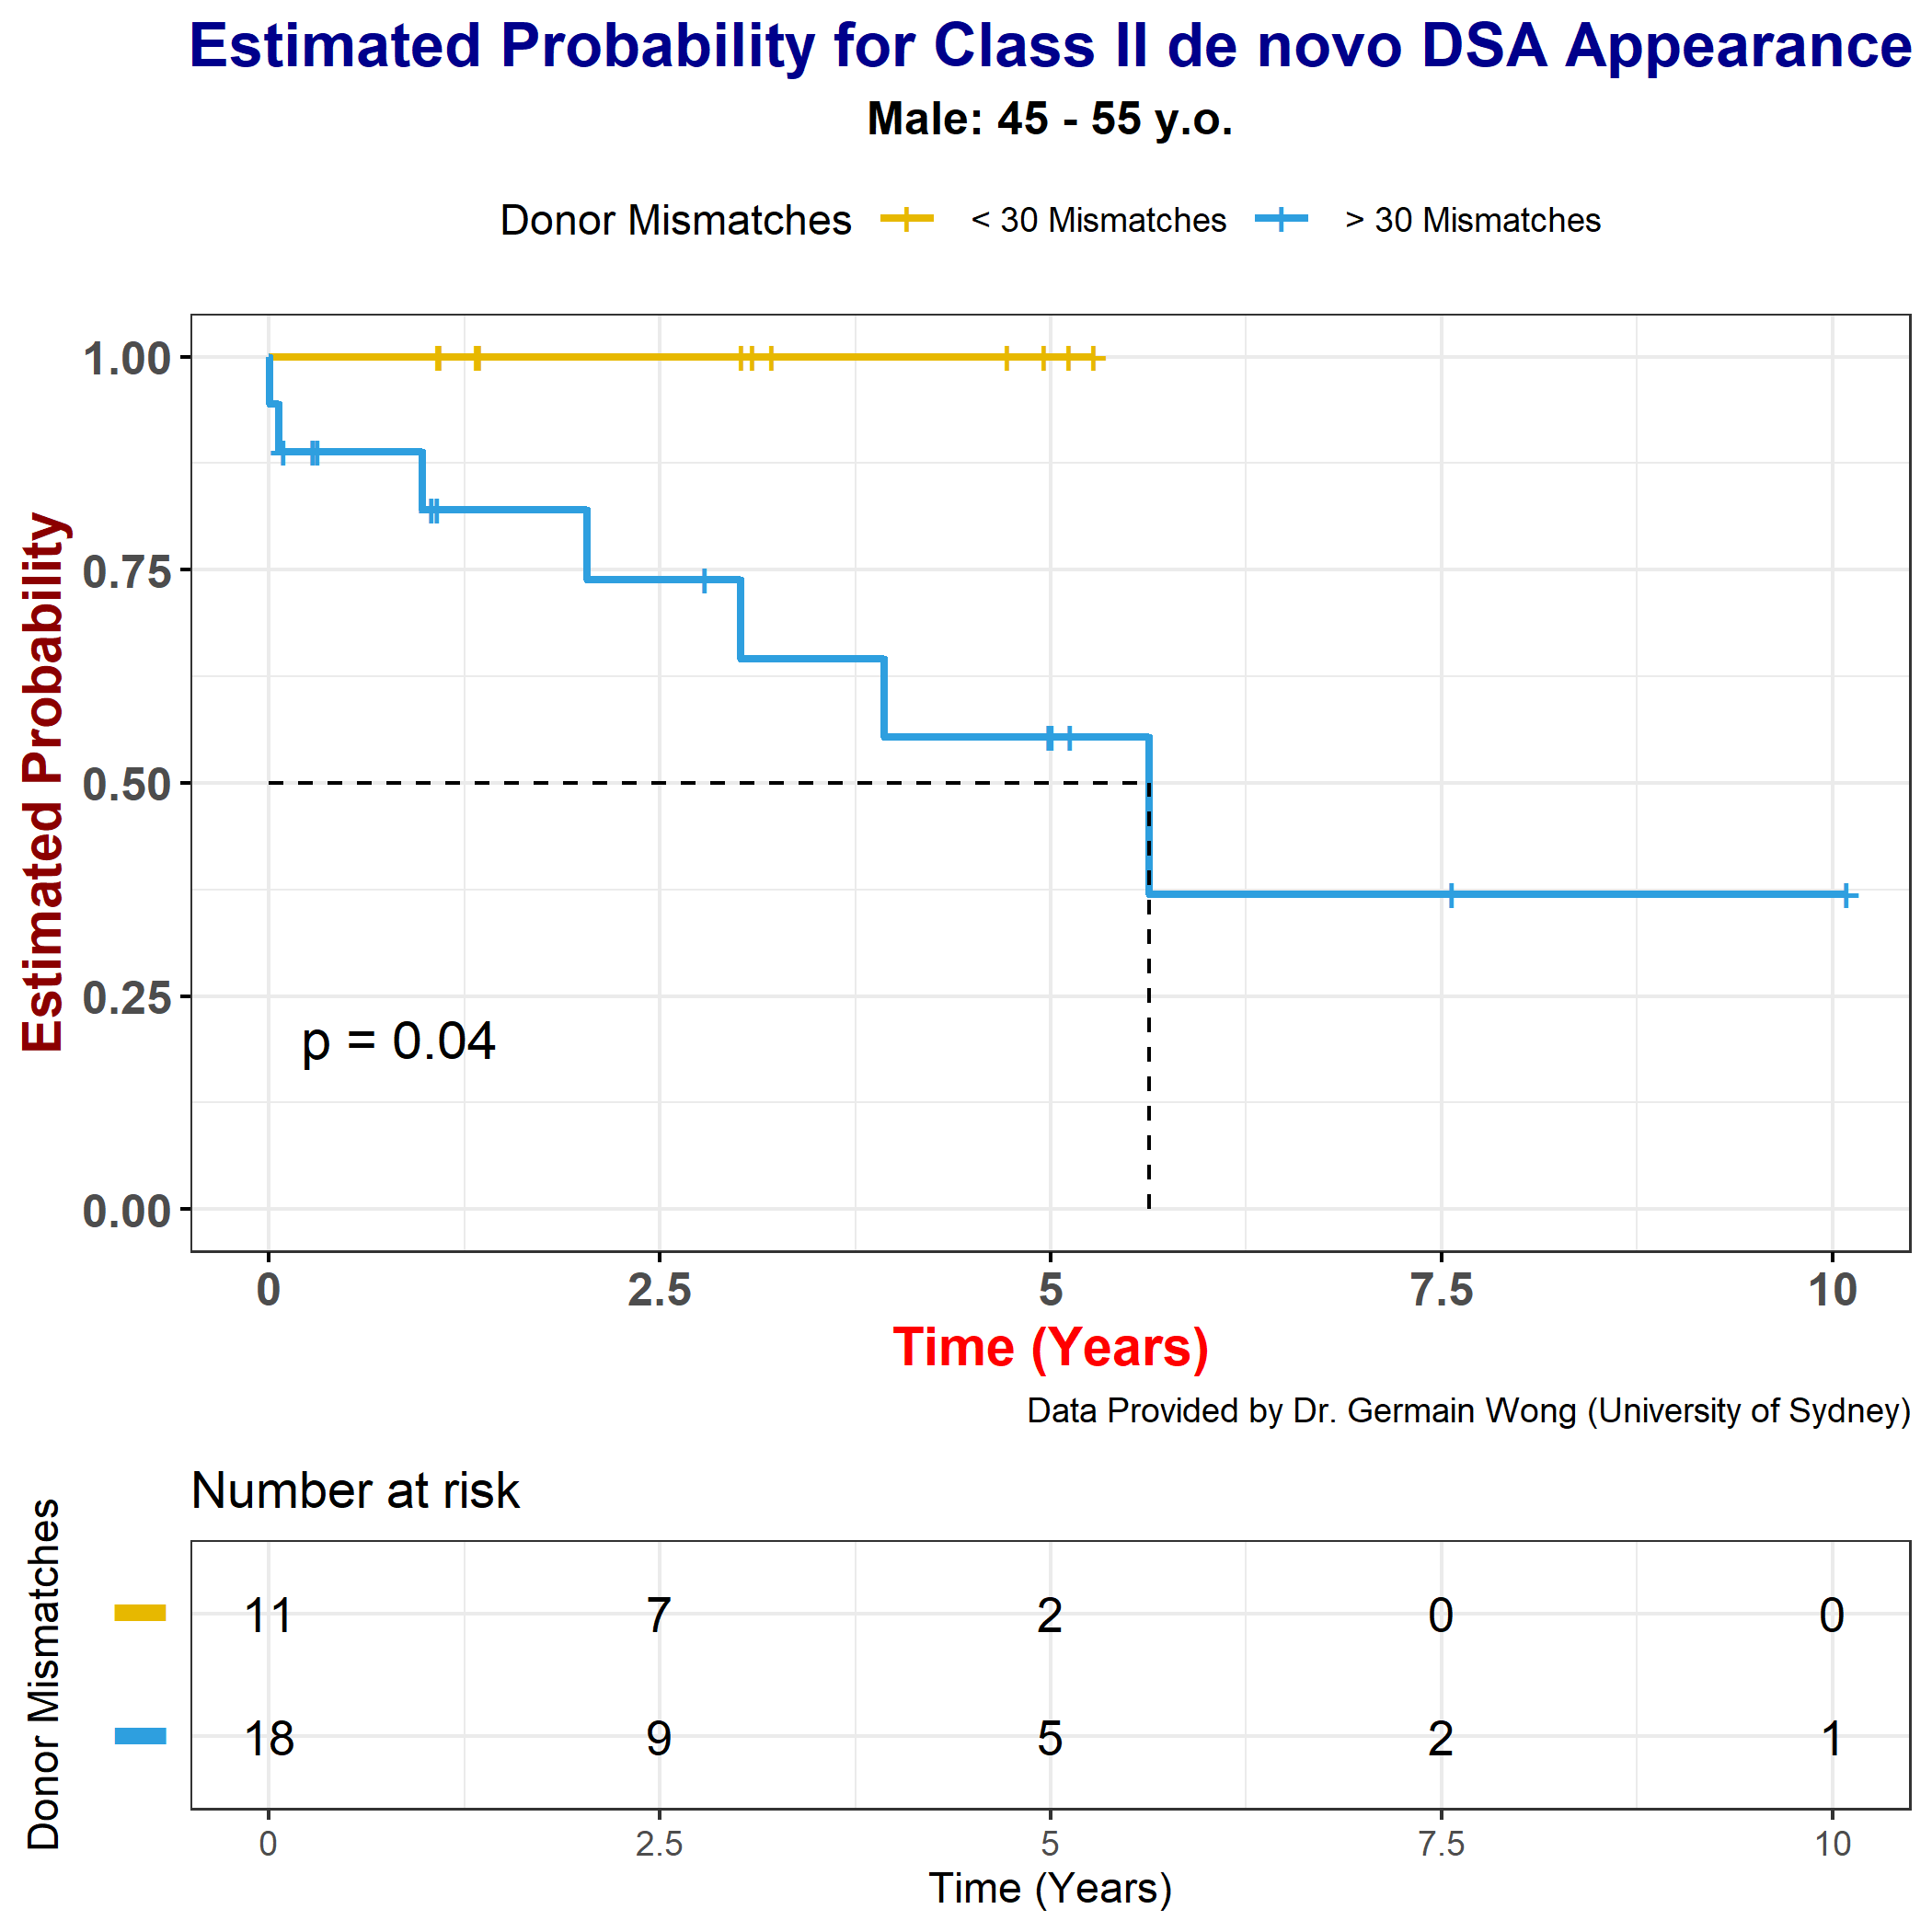
\includegraphics[width=200px]{images/part2survival} \end{center}

This may assist in better kidney allocation and prescriptions based on
historical performance of other recipients who belong to the same
subgroup.

\newpage

\hypertarget{discussion-and-conclusion}{%
\subsection{Discussion and Conclusion}\label{discussion-and-conclusion}}

\hypertarget{potential-shortcomings}{%
\subsubsection{Potential shortcomings}\label{potential-shortcomings}}

\hypertarget{shortcomings-with-part-1-predicting-ar}{%
\paragraph{Shortcomings with Part 1 (Predicting
AR)}\label{shortcomings-with-part-1-predicting-ar}}

The main shortcoming of the risk calculator is the long computational
time involved when the patient's input data is in the form of Ensembl ID
as it has to be converted to official gene symbols. Furthermore, if the
patient does not contain all 100 genes used to train the original model,
then the alternative model (as mentioned previously) must be made
on-demand, with computational times that can be rather long
(\textasciitilde{} 1 minute).

Furthermore, as demonstrated in the boxplot showing quantile-normalized
counts, the median of normalised gene expression in the training data is
around 10. This means that if the median of the input counts differs
significantly from 10, the prediction is likely to be invalid.

\hypertarget{shortcomings-with-part-2-estimating-dsa-presence}{%
\paragraph{Shortcomings with Part 2 (Estimating DSA
Presence)}\label{shortcomings-with-part-2-estimating-dsa-presence}}

The main shortcoming of this methodology is the use of a small dataset
(198 entries after removing null entries). Thus, when we stratify the
data based on subgroups of variables, we have limited information
available for creating the Kaplan Meier curve. Hence, some
subpopulations are inaccurately represented, with some curves being
uninformative.

Another shortcoming is the inability to verify if some positive events
(i.e.~DSA presence) were due to censoring or not. As such, this may
occasionally manifest as an overestimation in graft failure risk during
some periods.

\hypertarget{shortcomings-with-part-3-predicting-reliance-on-immunosuppression}{%
\paragraph{Shortcomings with Part 3 (Predicting Reliance on
Immunosuppression)}\label{shortcomings-with-part-3-predicting-reliance-on-immunosuppression}}

Similar to Part 1, limitations are primarily attributed to long
computational times for the same reasons.

However, an additional shortcoming with Part 3 is the small number of OT
patients (19) used to train the model. GSE2229 was one of the only
datasets with normalised OT gene expression able to be calculated, and
so the lack of data may diminish feasibility of predictions for patients
with gene expressions recorded from different platforms.

\hypertarget{future-work-and-improvements}{%
\subsubsection{Future work and
improvements}\label{future-work-and-improvements}}

The study of epitope compatibility is still in its infant stages and
hence, greater research needs to be taken in order to drive advancements
in ESRD management (Tambur 2018). Furthermore, a procedural standard in
experimental design is encouraged so that consistent results concerning
survivability can be reliably reproduced. For example, several studies
determining whether BMI is a significant variable for graft rejection
have demonstrated contradictory results, possibly due to different
experimental designs (Papalia et.al, 2010).

There is also a need for larger and more diverse datasets so that
various population confounders and other sources for variation can be
accounted for. For example, the eplet data consisted mostly of Caucasoid
patients, which could have affected graft outcome.

Finally, further study into operational tolerance (OT) may improve the
validity of future predictions as there are currently limited samples of
OT patients globally. Indeed, OT diagnosis is difficult due to the
ethical issues of temporarily ceasing immunosuppressive therapy.

\hypertarget{conclusion}{%
\subsubsection{Conclusion}\label{conclusion}}

In conclusion, we believe the risk calculator will aid in the effective
and accurate allocation of kidney donor organs to those needing the
lifesaving treatment of transplantation. In particular, by predicting a
patient's graft outcome in terms of AR, OT, and estimated time until DSA
appear (in relation to the sub-population corresponding to their
phenotype), we hope that we can assist practitioners in their
decision-making and make more informed choices in immunosuppressive
prescriptions.

\newpage

\hypertarget{reference-list}{%
\subsection{Reference List}\label{reference-list}}

Australian Institute of Health and Welfare. (2019) Chronic Kidney
Disease. Retrieved from
\url{https://www.aihw.gov.au/reports-data/health-conditions-disability-deaths/chronic-kidney-disease/overview}

Dayoub, J. C., Cortese, F., Anzic, A., Grum, T., \& de Magalhaes, J. P.
(2018). The effects of donor age on organ transplants: A review and
implications for aging research. Experimental gerontology, 110, 230-240.

Edgar R., Domrachev M., Lash AE. (2002). Gene Expression Omnibus: NCBI
gene expression and hybridization array data repository. Nucleic Acids
Res, 30(1),207-10.

Gordon, E. J., Butt, Z., Jensen, S. E., Lok‐Ming Lehr, A., Franklin, J.,
Becker, Y., \ldots{} \& Penrod, D. (2013). Opportunities for shared
decision making in kidney transplantation. American Journal of
Transplantation, 13(5), 1149-1158.

David, G., \& Kleinbaum, K. (2016). Survival analysis: a self-learning
text. Springer-Verlag New York.

Law, C. W., Alhamdoosh, M., Su, S., Dong, X., Tian, L., Smyth, G. K., \&
Ritchie, M. E. (2016). RNA-seq analysis is easy as 1-2-3 with limma,
Glimma and edgeR. F1000Research, 5.

Massart, A., Ghisdal, L., Abramowicz, M., \& Abramowicz, D. (2017).
Operational tolerance in kidney transplantation and associated
biomarkers. Clinical \& Experimental Immunology, 189(2), 138-157.

Menon, M. C., Cravedi, P., \& El Salem, F. (2017). Acute Cellular
Rejection. In Kidney Transplantation, Bioengineering and Regeneration
(pp.~461-474). Academic Press.

Newell, K. A., Adams, A. B., \& Turka, L. A. (2018). Biomarkers of
operational tolerance following kidney transplantation--The immune
tolerance network studies of spontaneously tolerant kidney transplant
recipients. Human immunology, 79(5), 380-387.

Papalia, T., Greco, R., Lofaro, D., Maestripieri, S., Mancuso, D., \&
Bonofiglio, R. (2010). Impact of body mass index on graft loss in normal
and overweight patients: retrospective analysis of 206 renal
transplants. Clinical transplantation, 24(6), E241--E246.

Tambur, A. R. (2018). HLA-epitope matching or eplet risk stratification:
the devil is in the details. Frontiers in immunology, 9, 2010.

Qiu, X., Wu, H. \& Hu, R. The impact of quantile and rank normalization
procedures on the testing power of gene differential expression
analysis. BMC Bioinformatics 14, 124 (2013).

\newpage
\newpage

\hypertarget{appendix}{%
\subsection{Appendix}\label{appendix}}

\hypertarget{appendix-1.-ridge-and-lasso-results-for-part-1}{%
\subsubsection{Appendix 1. Ridge and LASSO results for Part
1}\label{appendix-1.-ridge-and-lasso-results-for-part-1}}

\begin{center}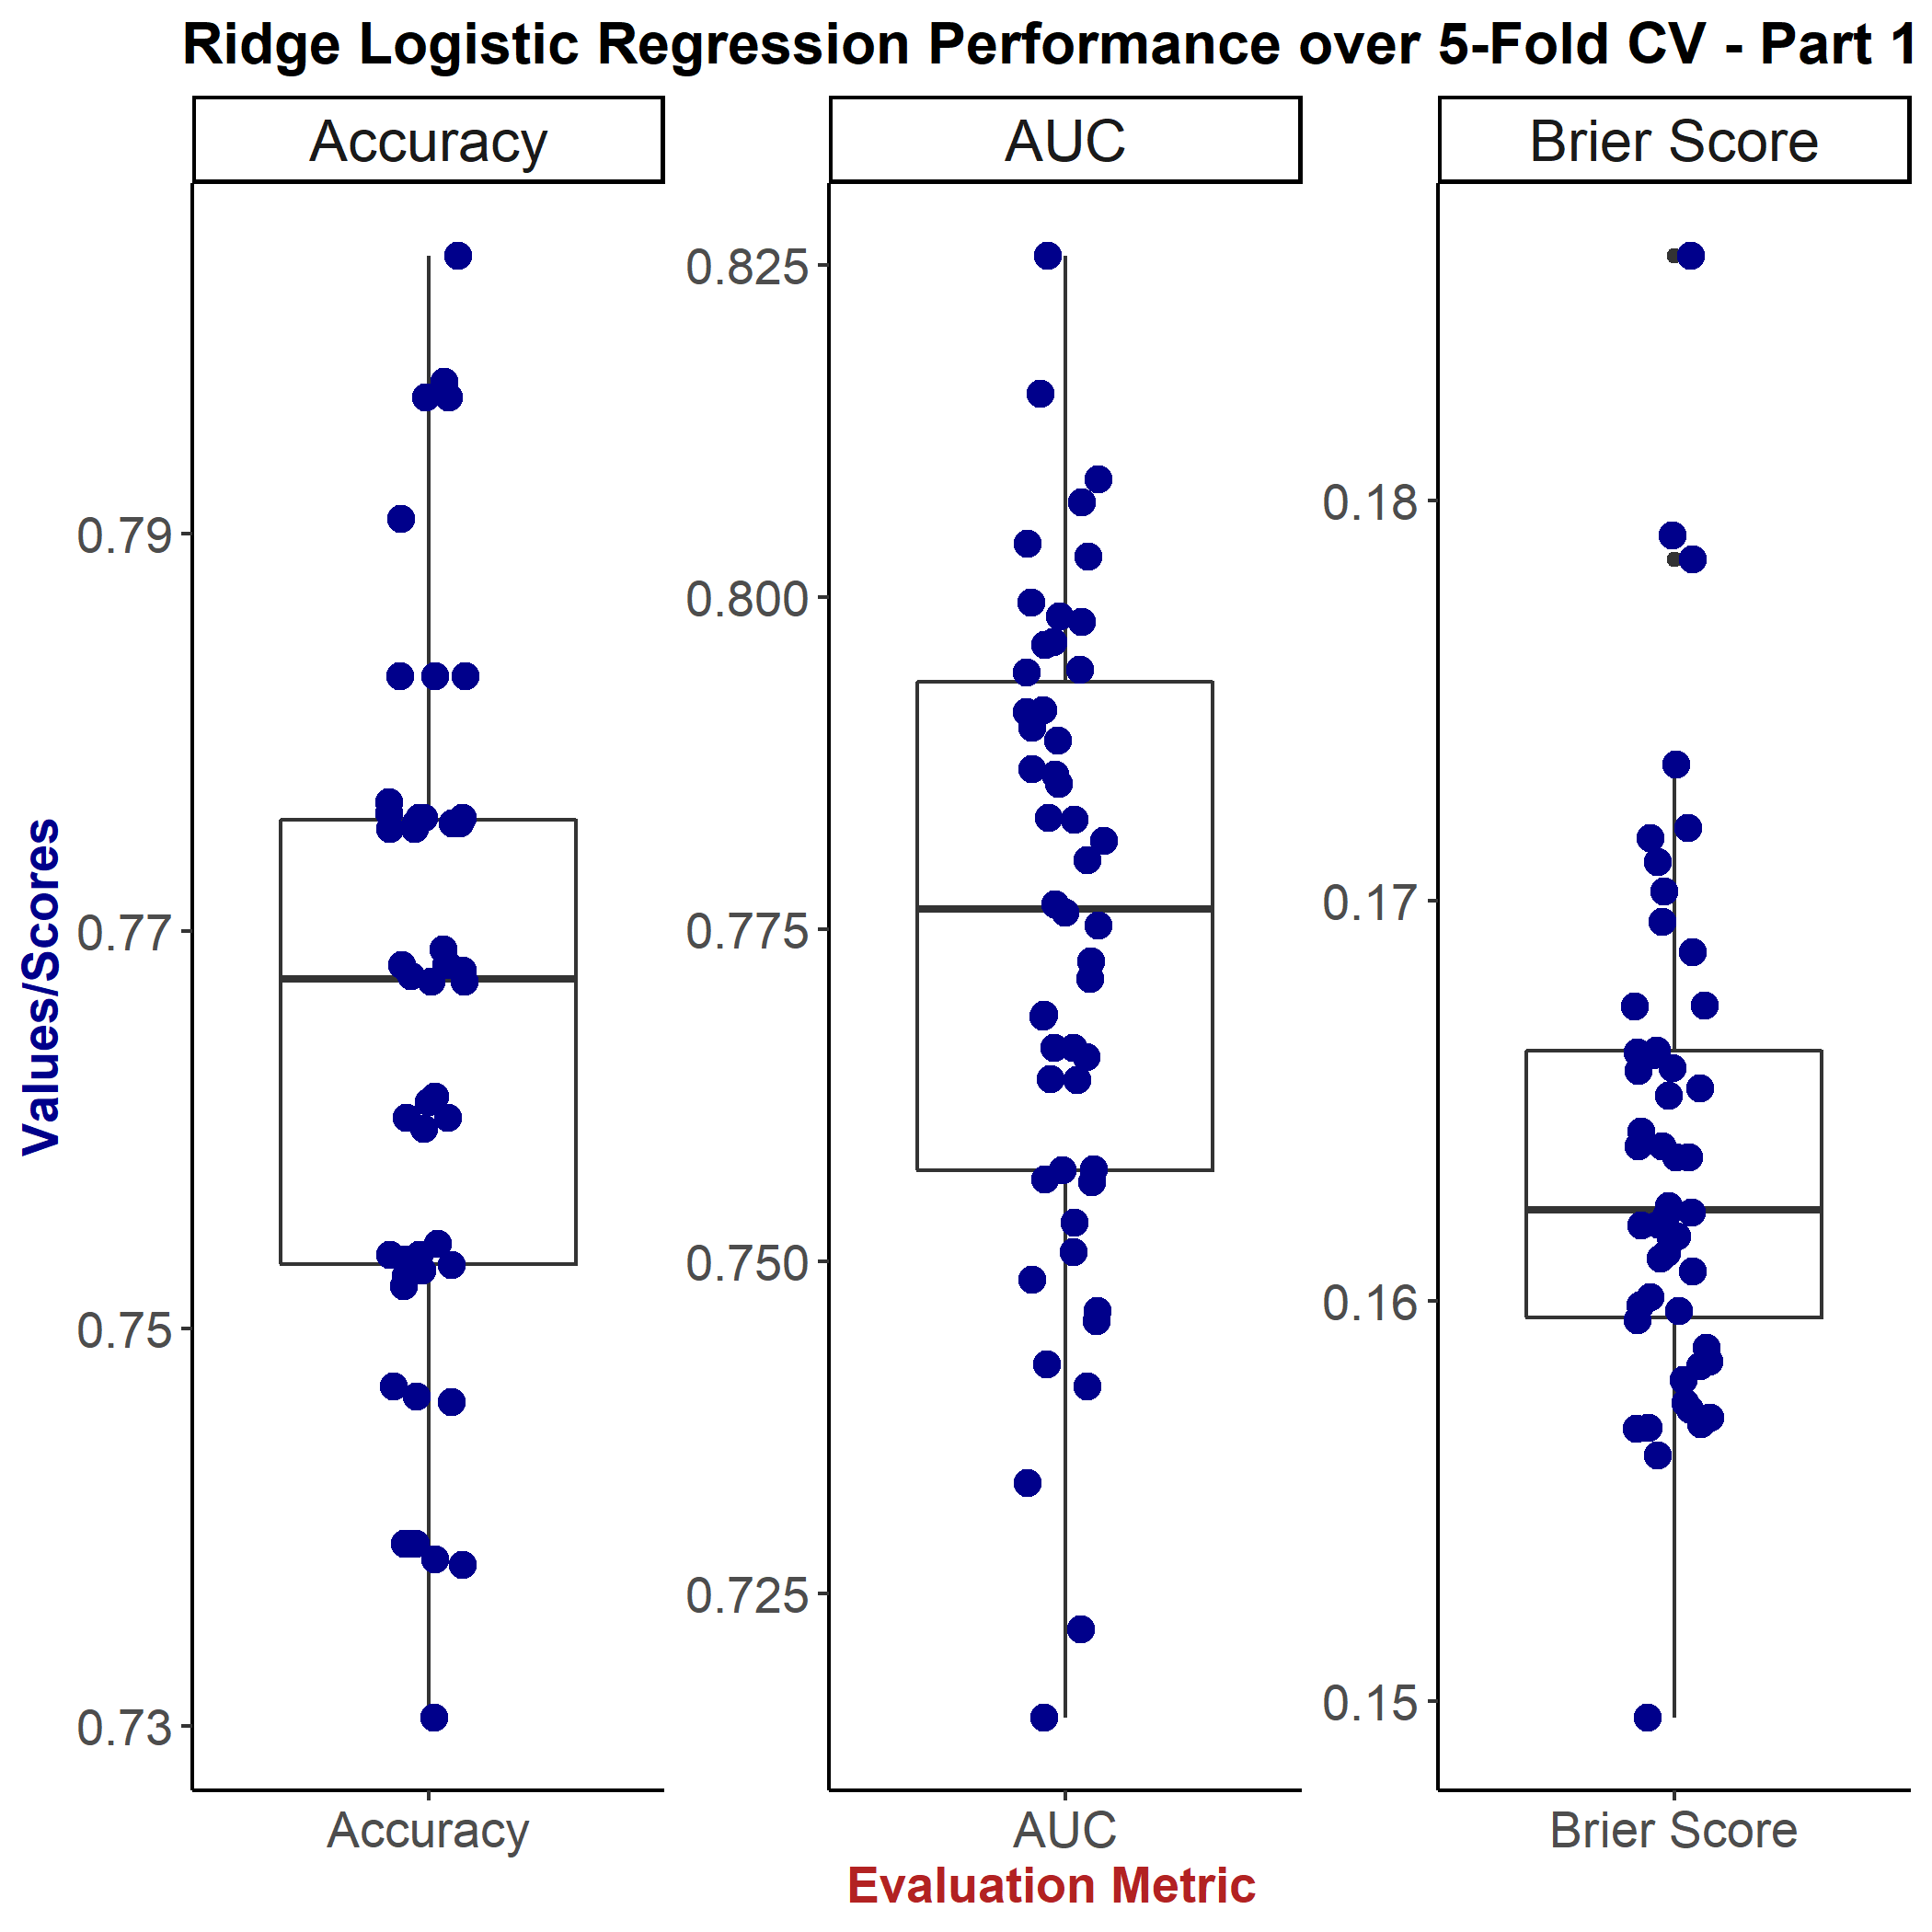
\includegraphics[width=220px]{images/part1ridge} \end{center}

\begin{center}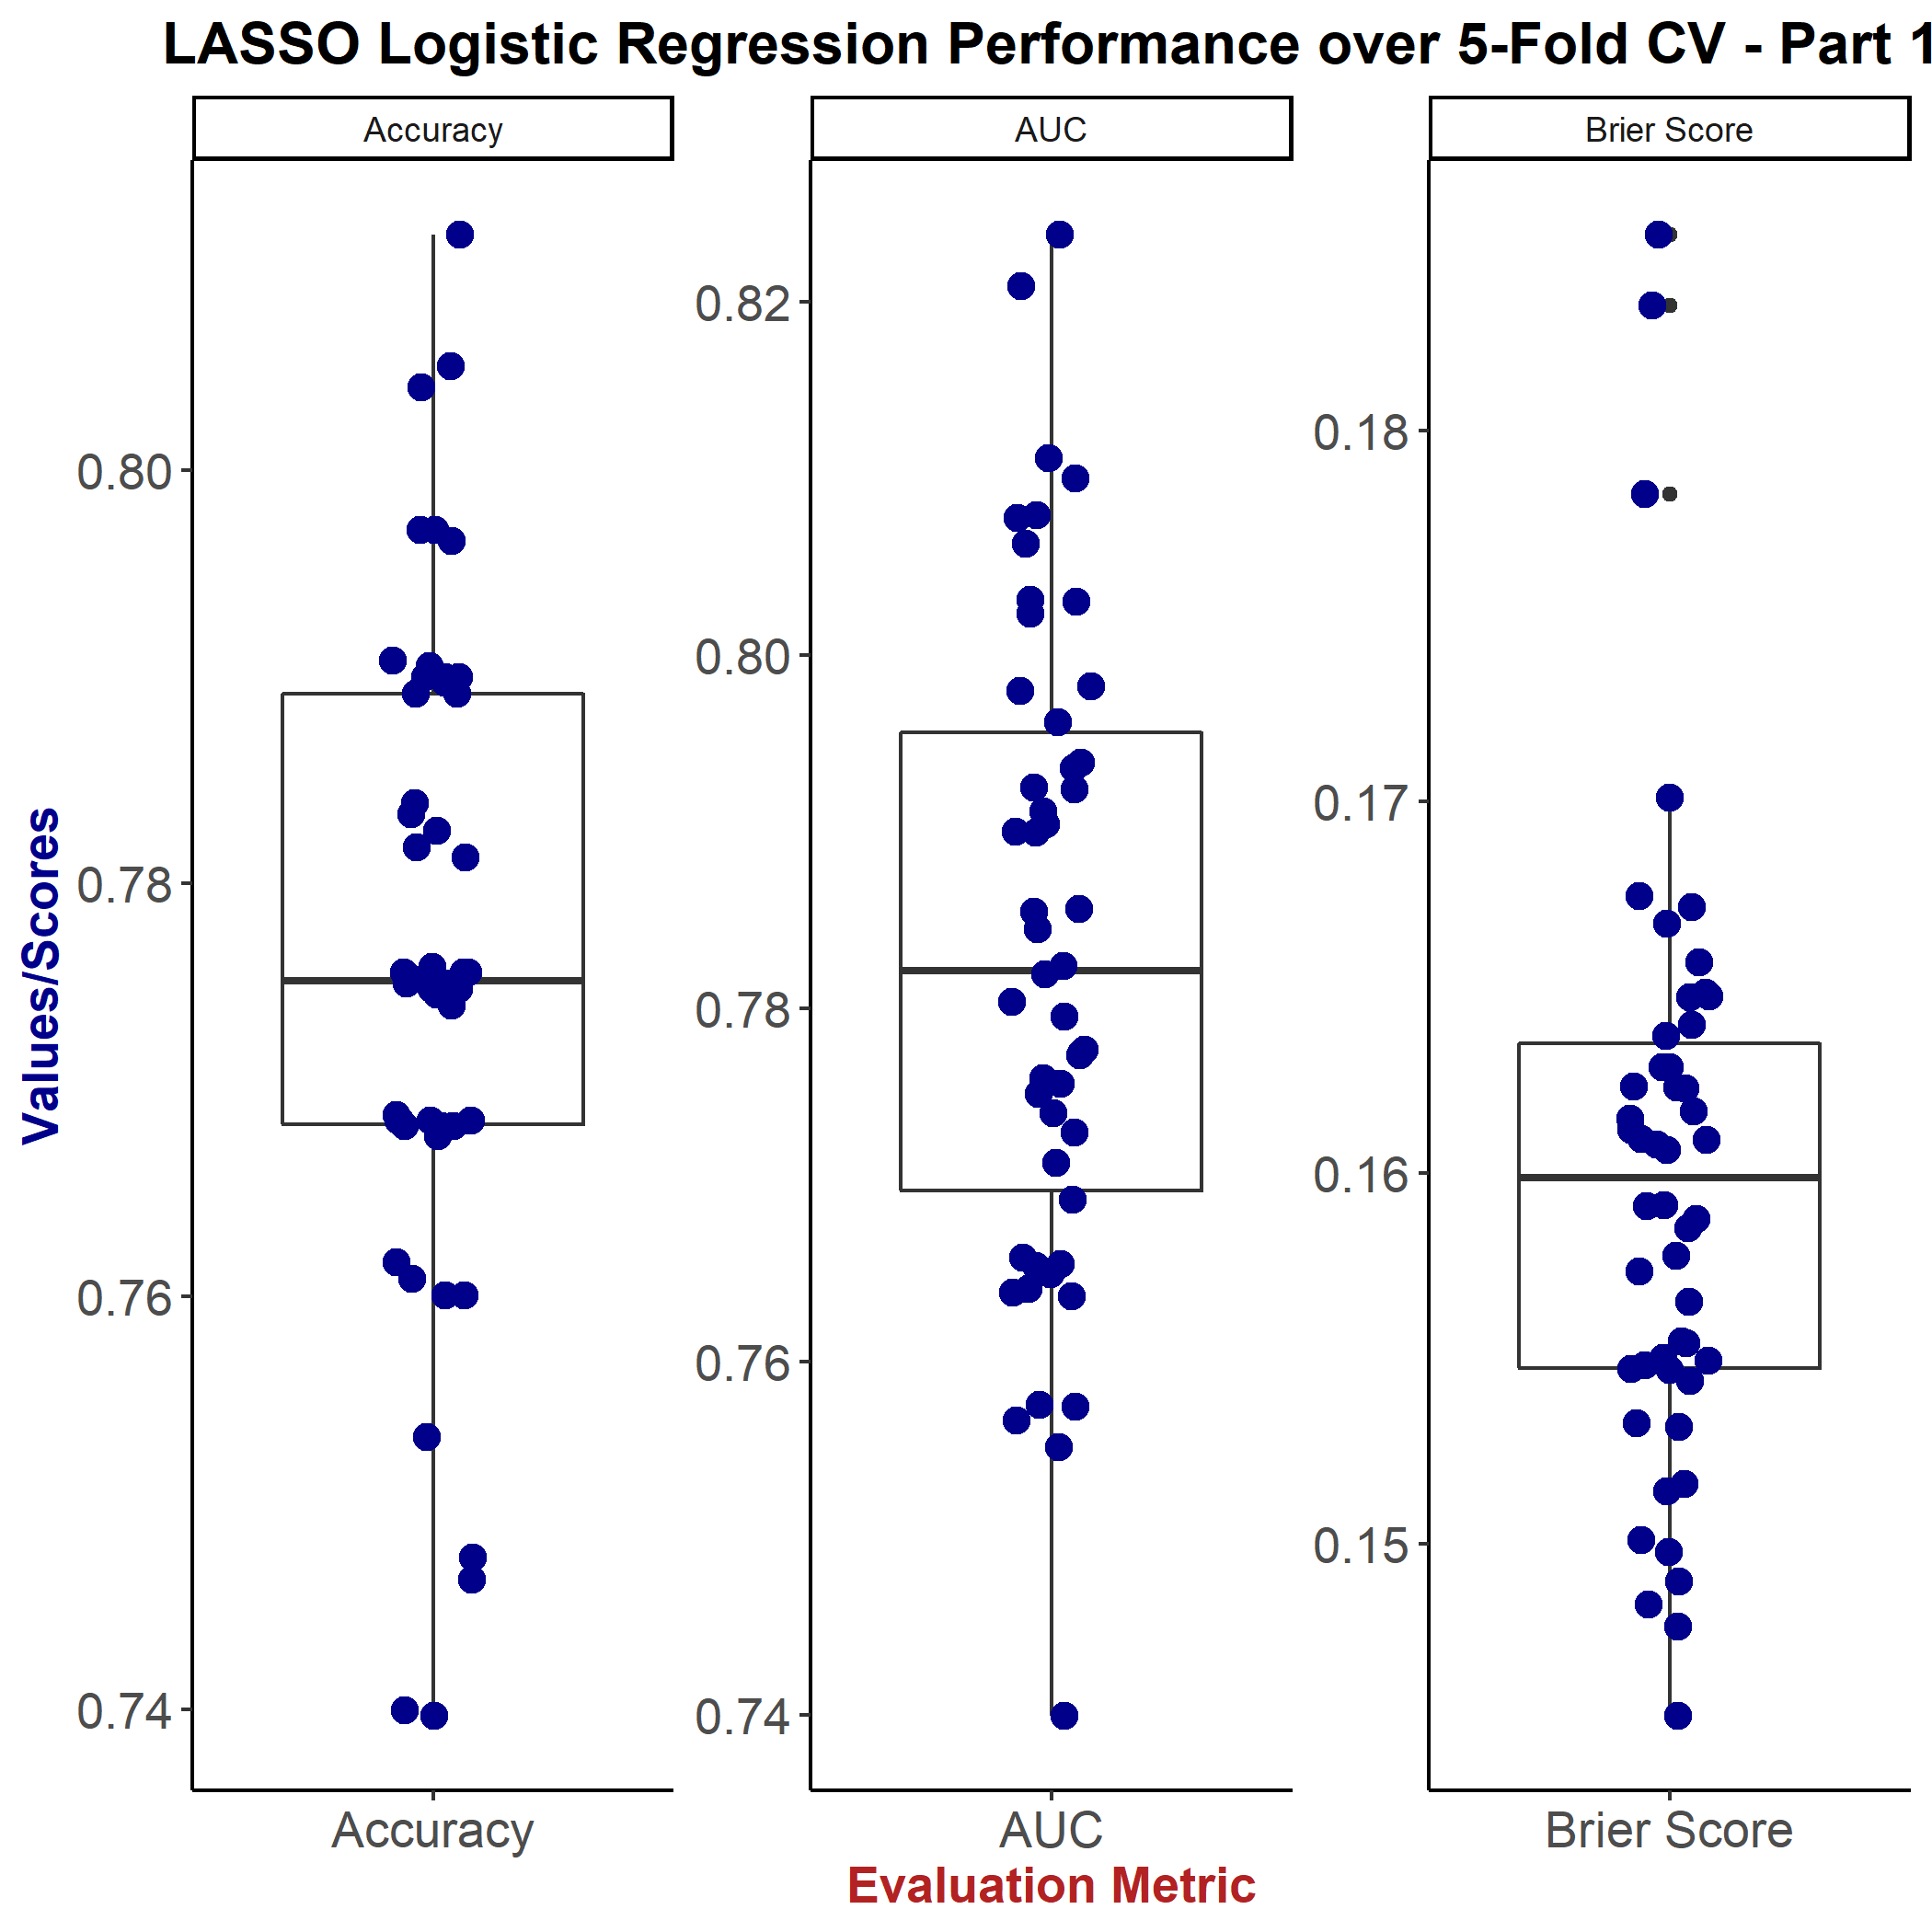
\includegraphics[width=220px]{images/part1lasso} \end{center}

\hypertarget{appendix-2.-ridge-and-lasso-results-for-part-3}{%
\subsubsection{Appendix 2. Ridge and LASSO results for Part
3}\label{appendix-2.-ridge-and-lasso-results-for-part-3}}

\begin{center}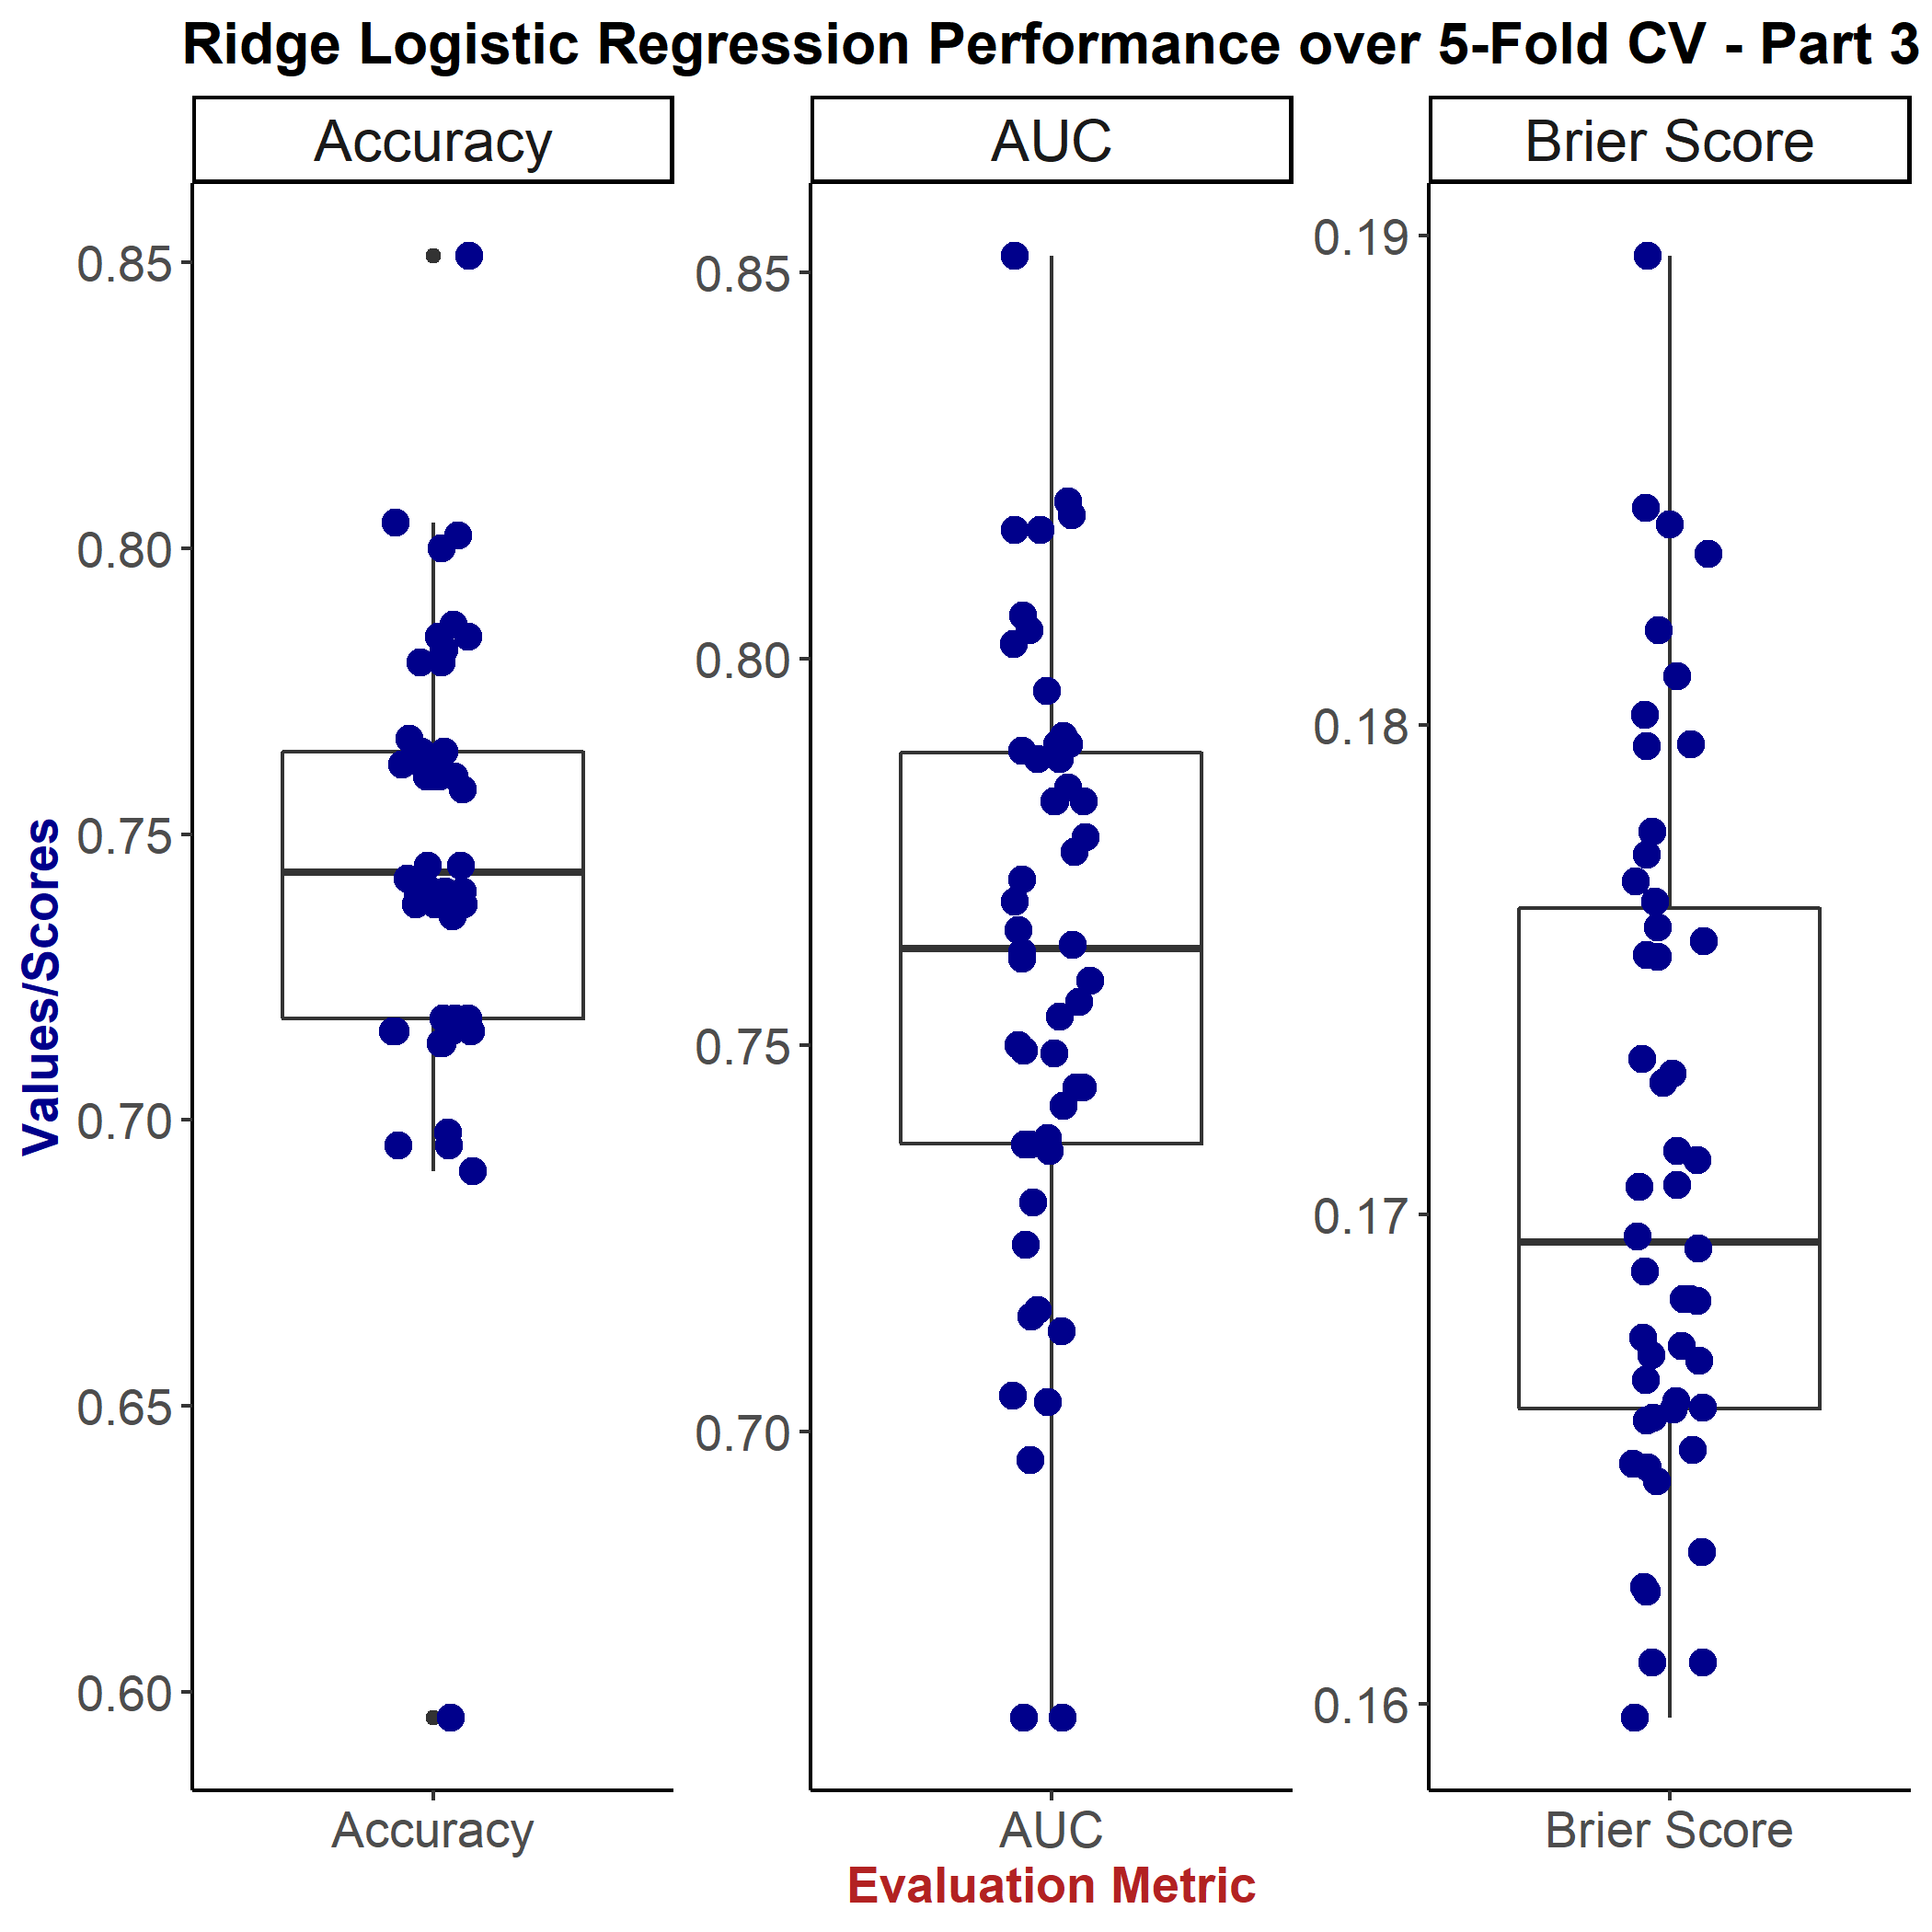
\includegraphics[width=220px]{images/part3ridge} \end{center}

\begin{center}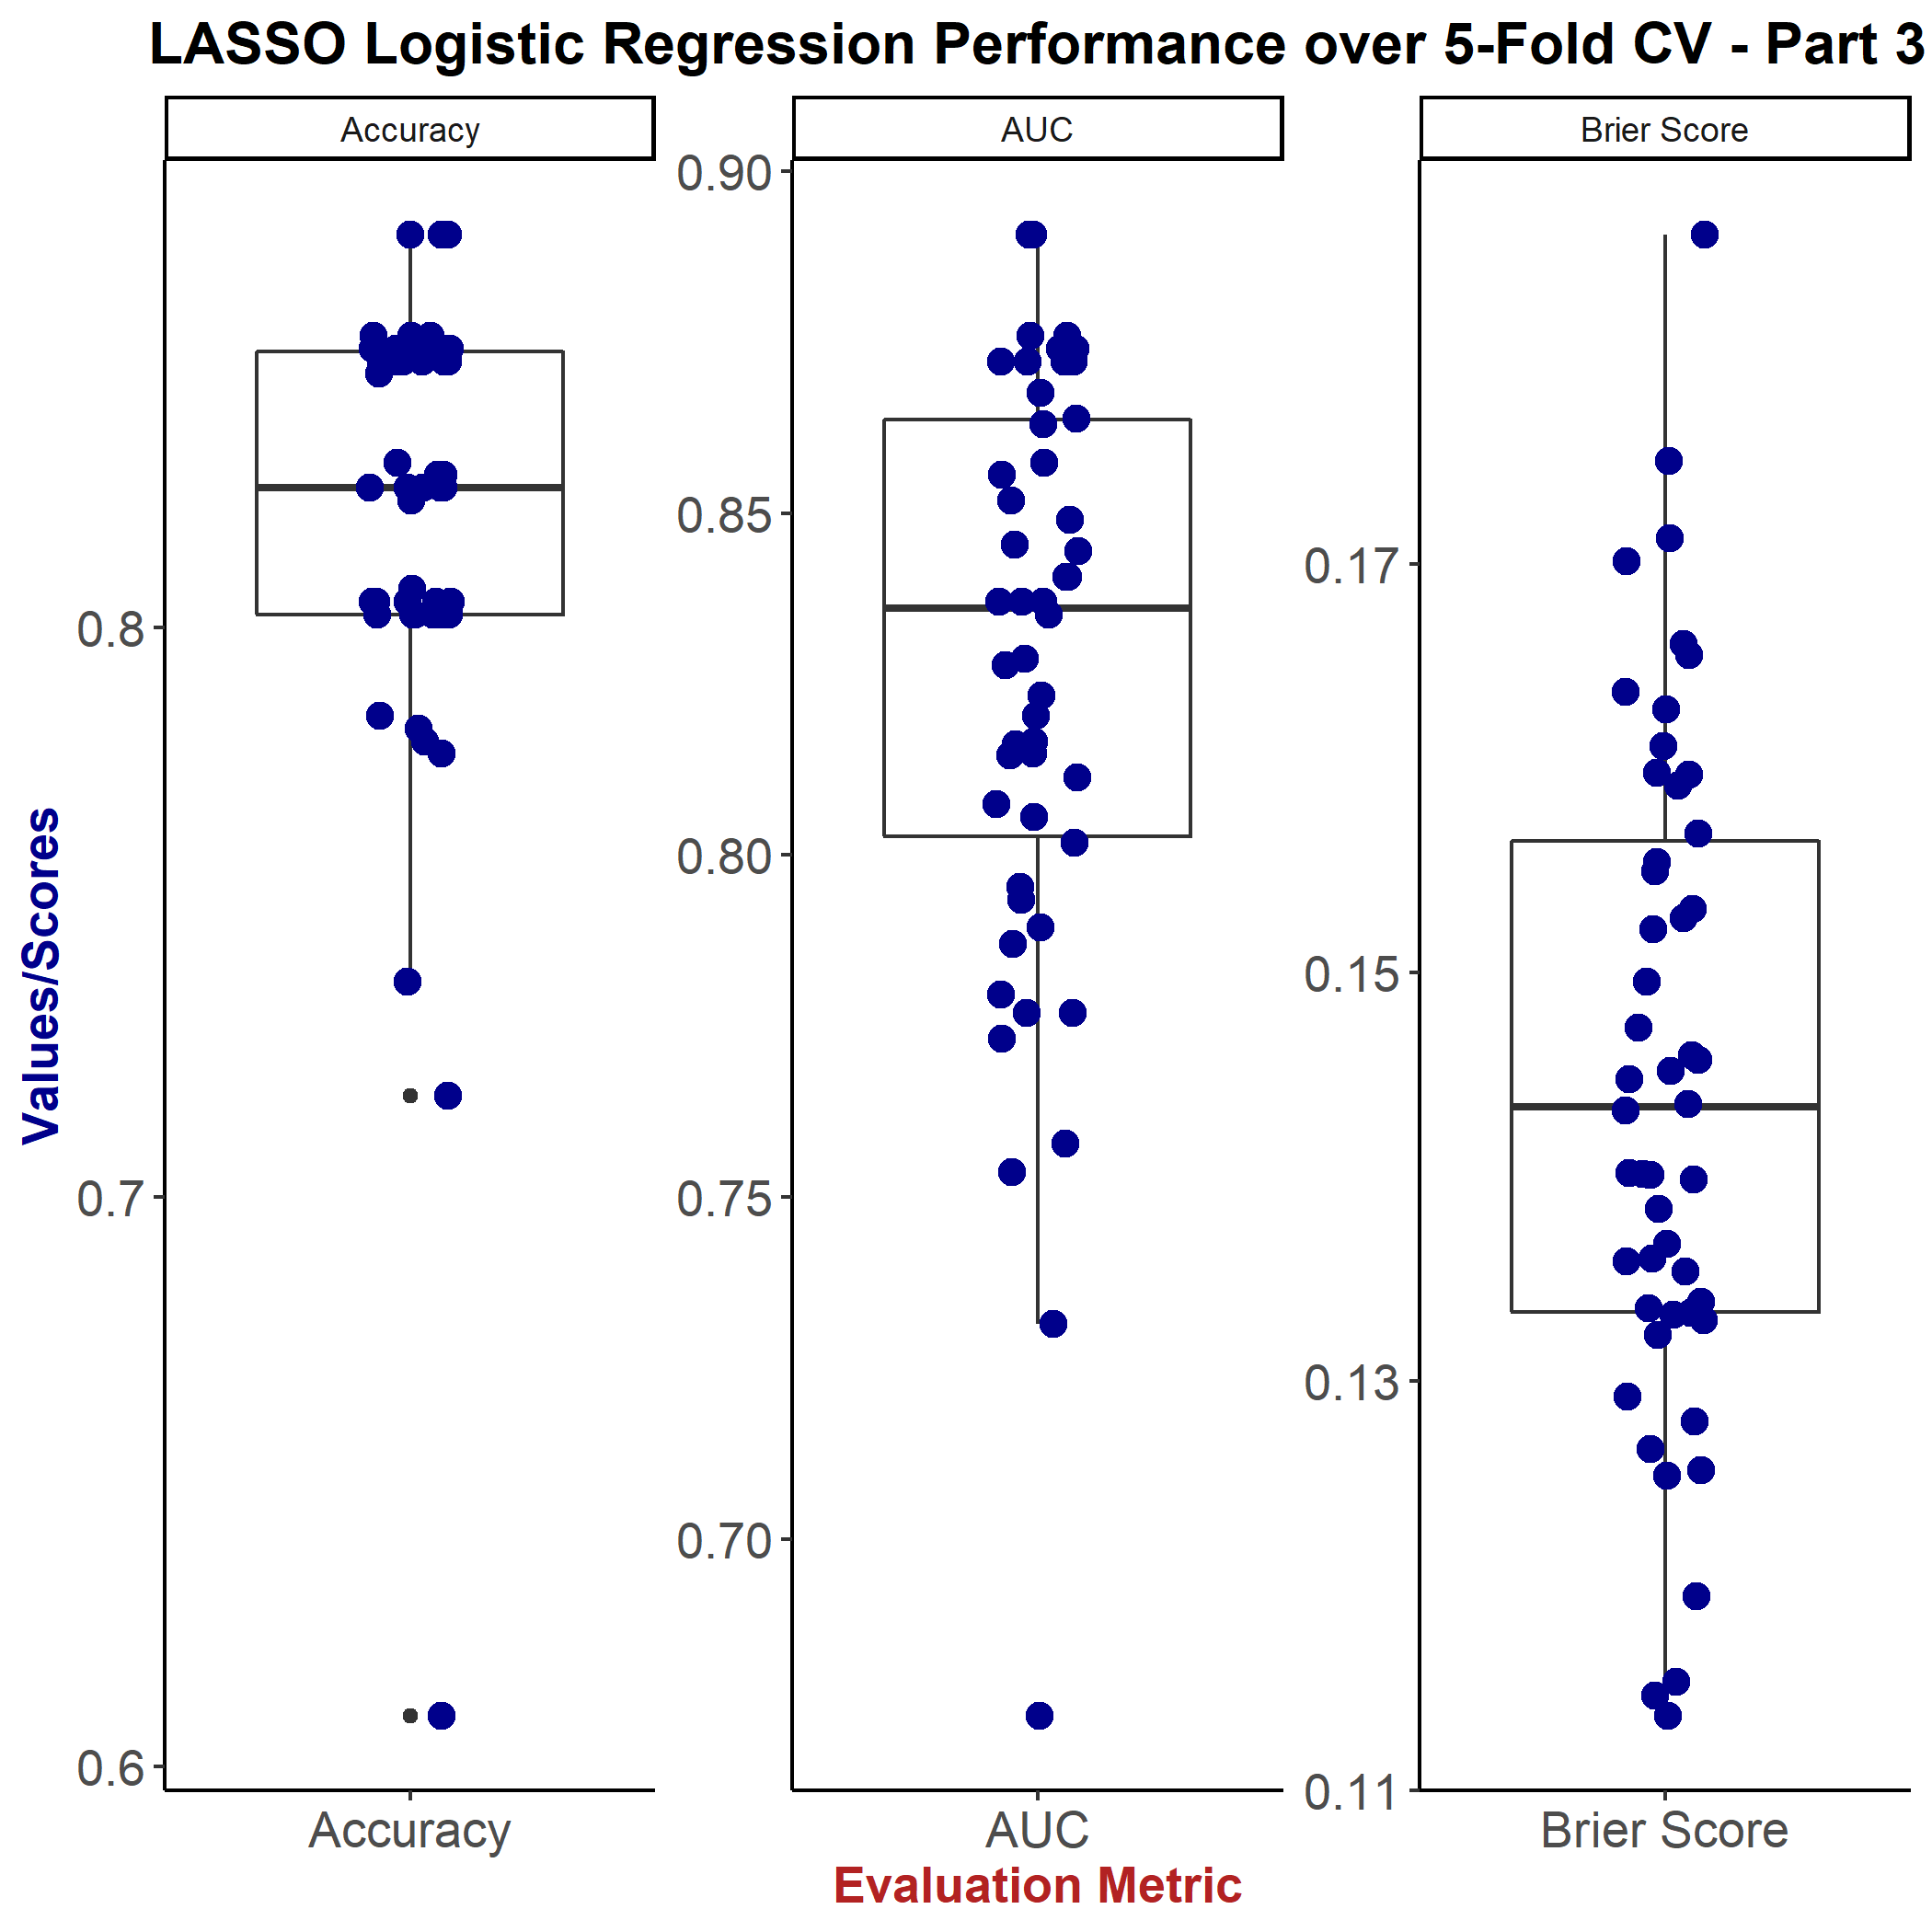
\includegraphics[width=220px]{images/part3lasso} \end{center}

\hypertarget{appendix-3.-gauge-plot-result-in-predicting-immunosuppresion-reliance}{%
\subsubsection{Appendix 3. Gauge Plot result in Predicting
Immunosuppresion
Reliance}\label{appendix-3.-gauge-plot-result-in-predicting-immunosuppresion-reliance}}

\begin{center}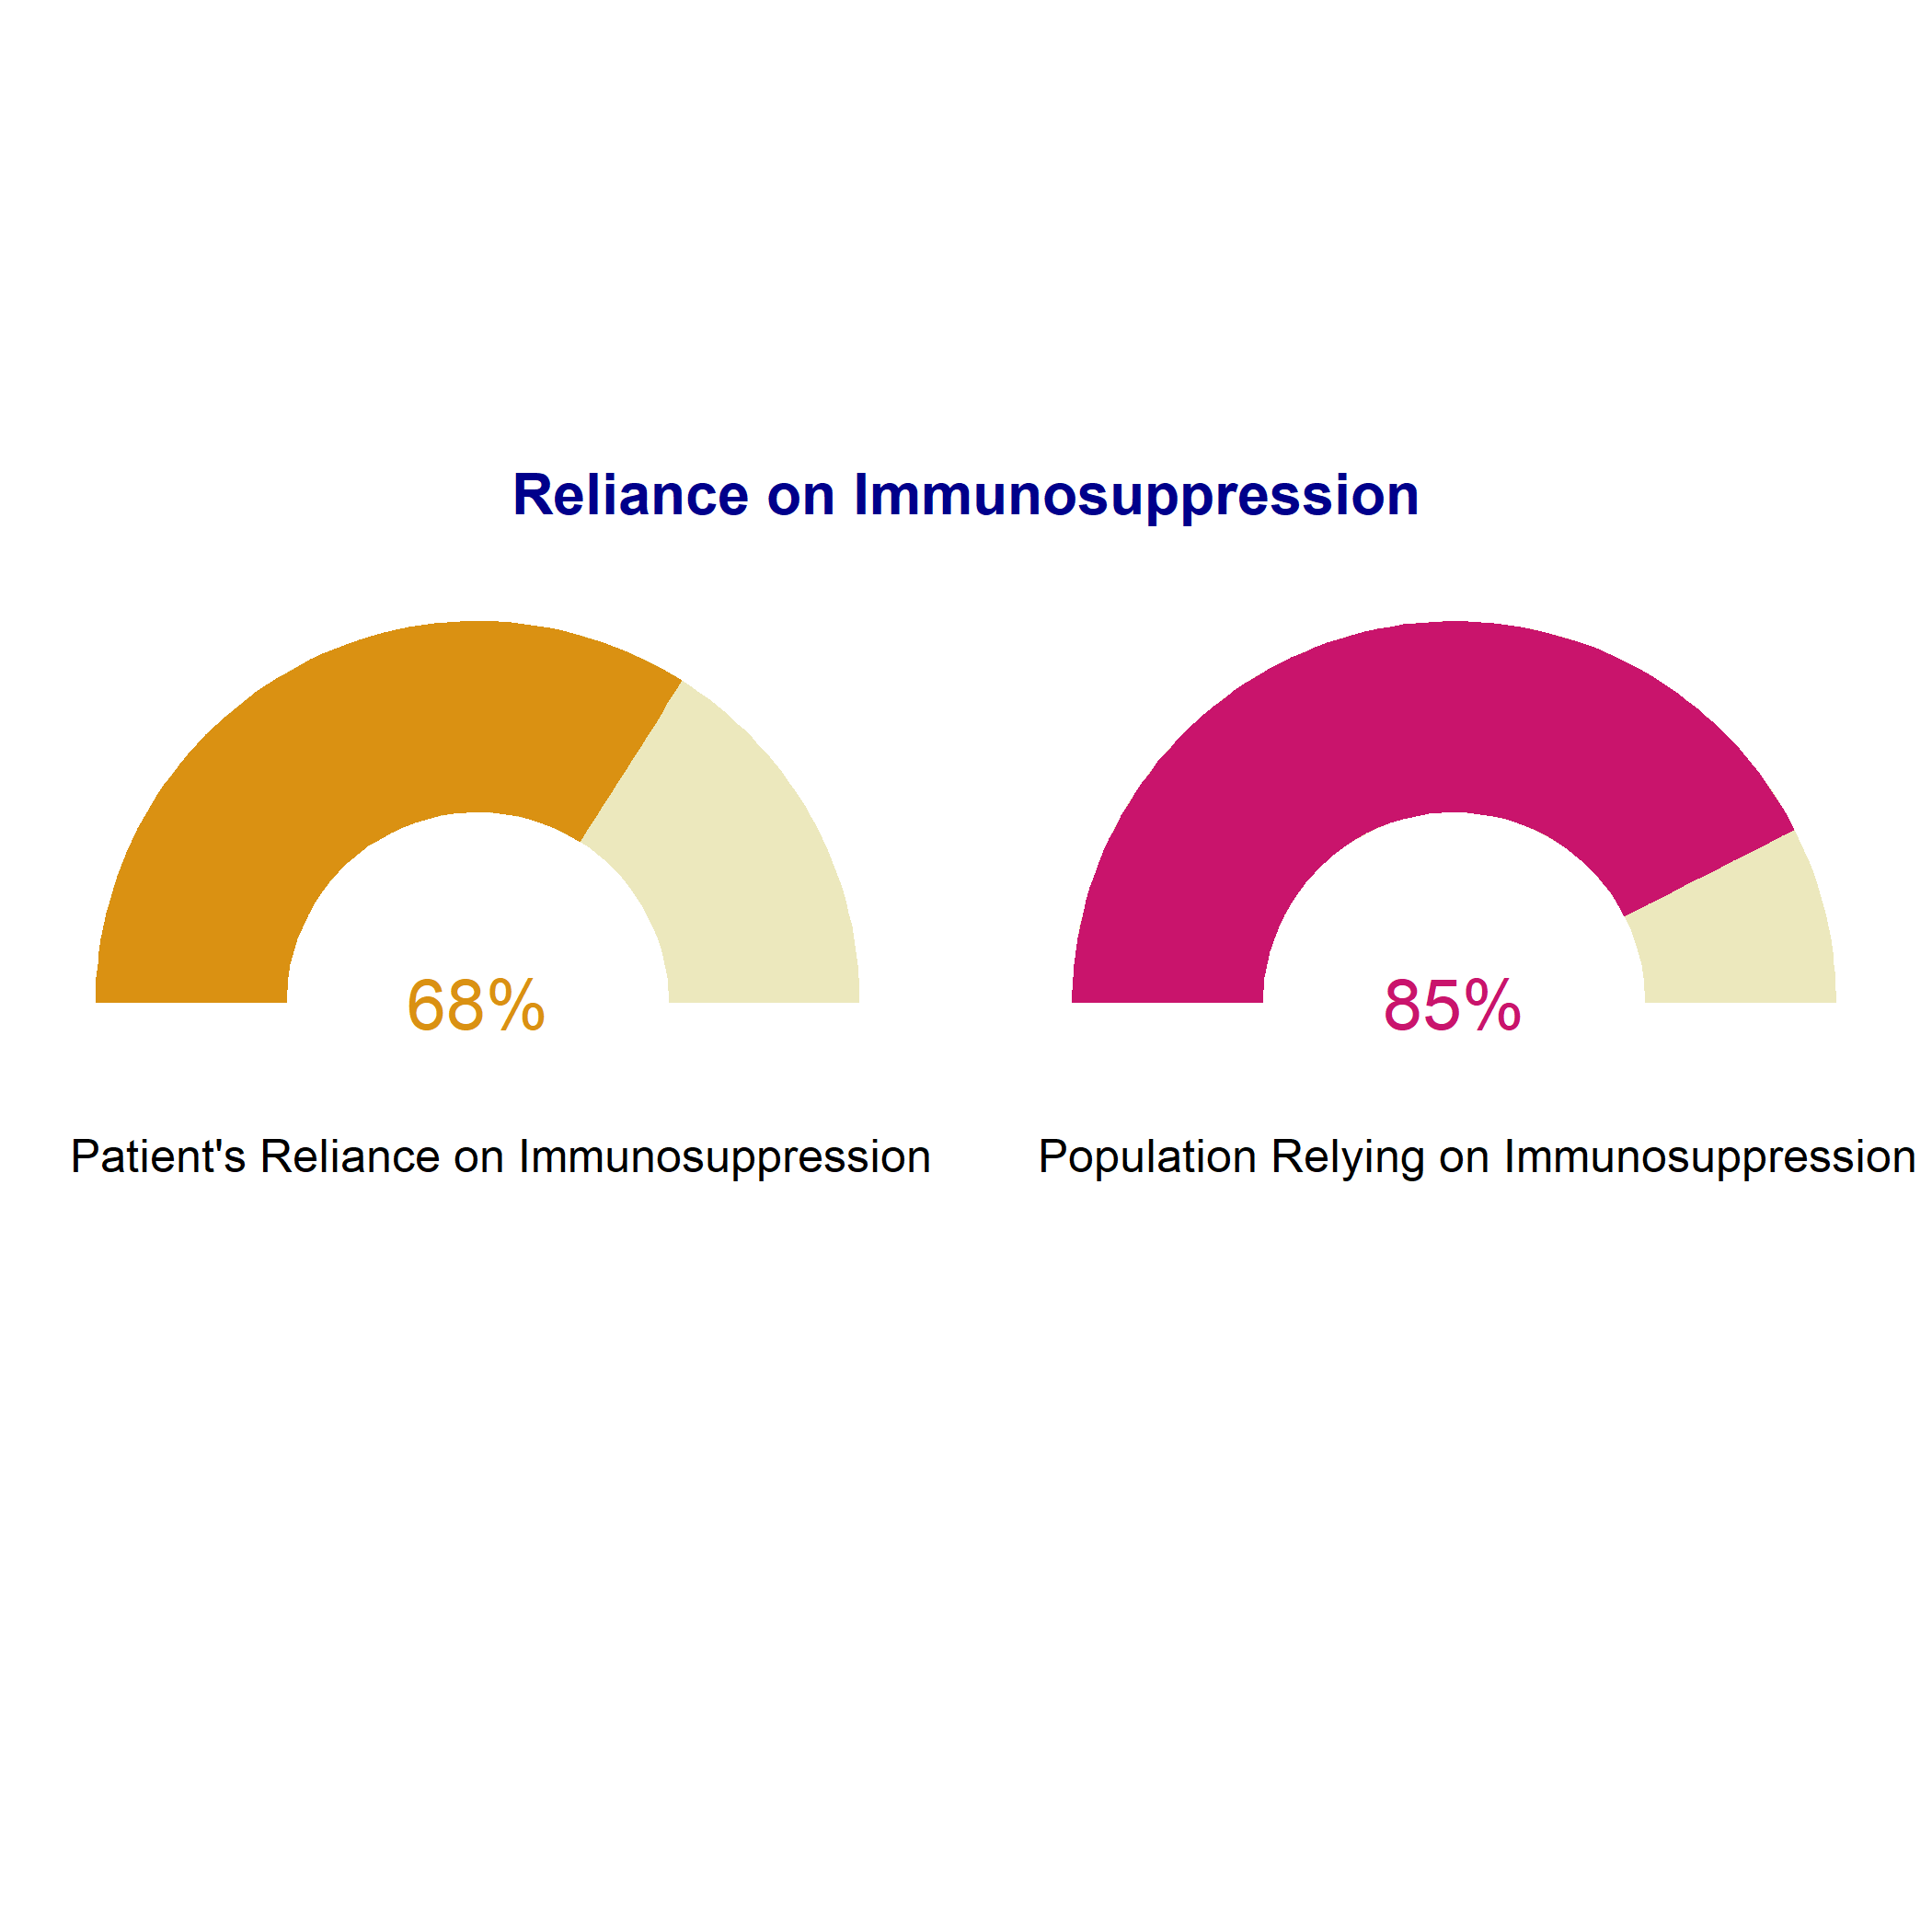
\includegraphics[width=220px]{images/part3_gauge} \end{center}

\newpage

\hypertarget{appendix-4.-patient-input-from-shiny-application}{%
\subsubsection{Appendix 4. Patient Input from Shiny
Application}\label{appendix-4.-patient-input-from-shiny-application}}

\begin{center}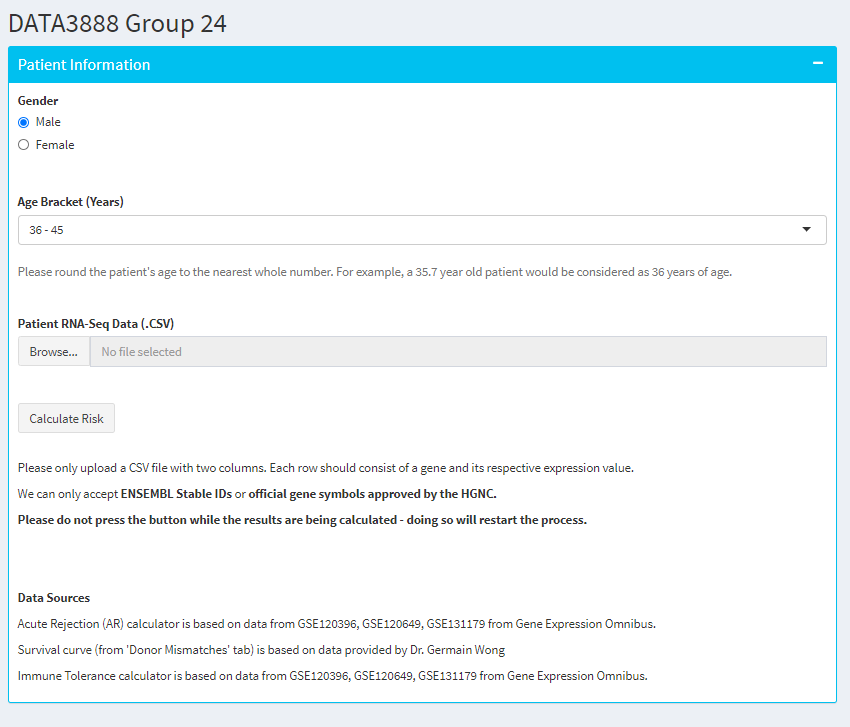
\includegraphics[width=250px]{images/PatientInput} \end{center}

\hypertarget{appendix-5.-information-tab-from-shiny-application}{%
\subsubsection{Appendix 5. Information Tab from Shiny
Application}\label{appendix-5.-information-tab-from-shiny-application}}

\begin{center}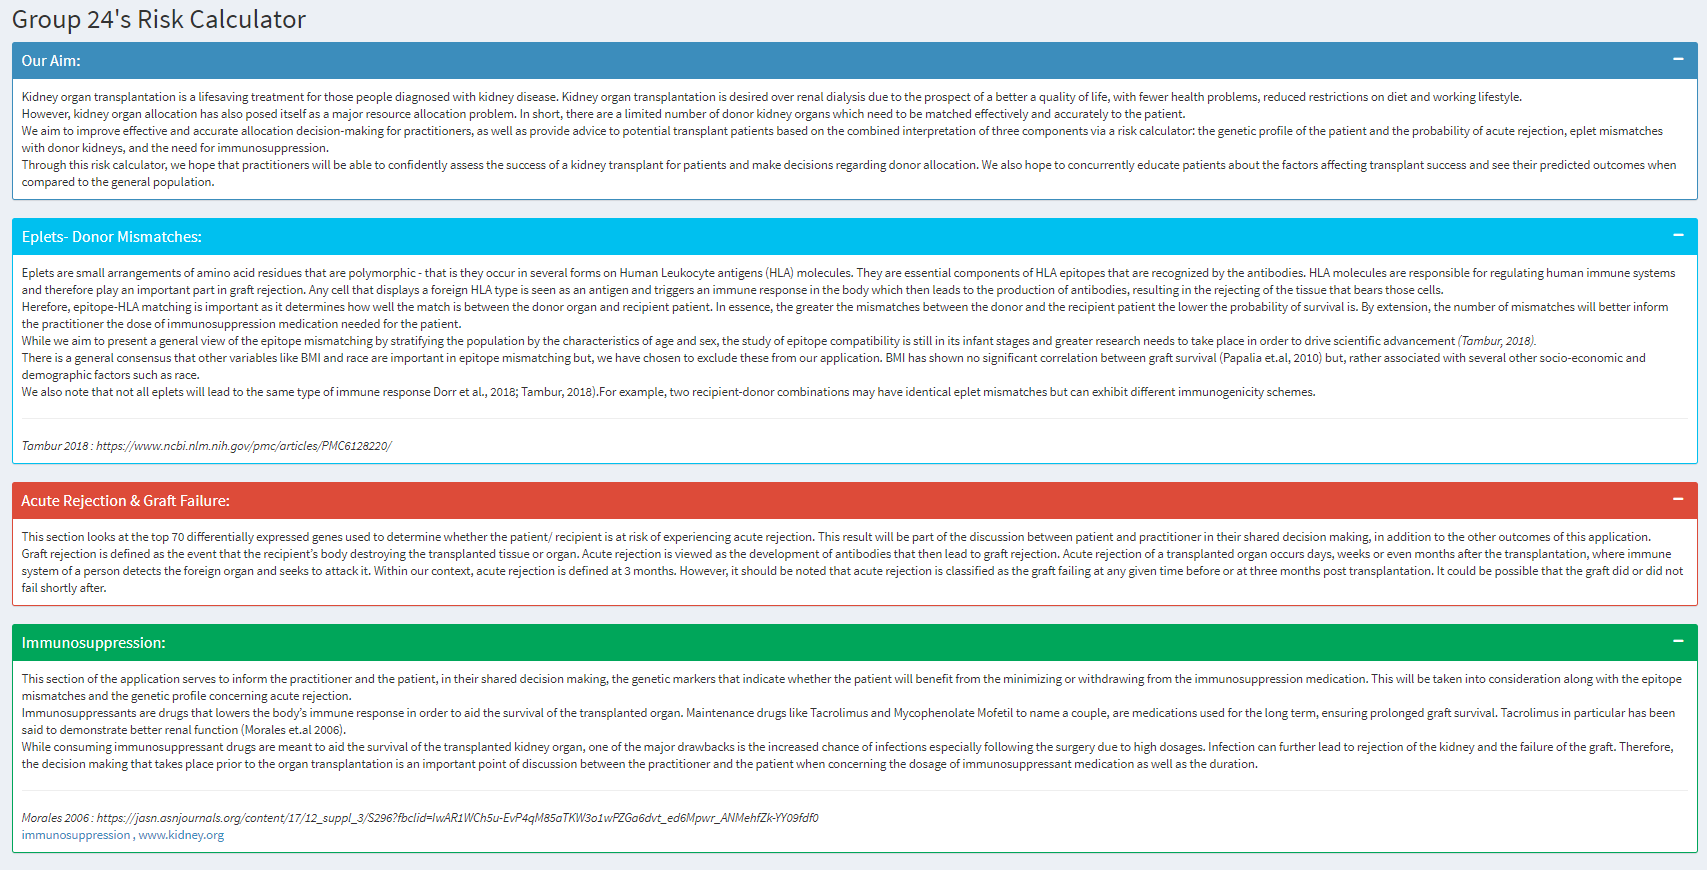
\includegraphics[width=250px]{images/Information} \end{center}

%\showmatmethods


\bibliography{pinp}
\bibliographystyle{jss}



\end{document}

